% Options for packages loaded elsewhere
\PassOptionsToPackage{unicode}{hyperref}
\PassOptionsToPackage{hyphens}{url}
%
\documentclass[
]{book}
\title{My First Steps in Neuronal Networks\\
(Beginners Guide)}
\author{Axel Roth}
\date{2021-11-11}

\usepackage{amsmath,amssymb}
\usepackage{lmodern}
\usepackage{iftex}
\ifPDFTeX
  \usepackage[T1]{fontenc}
  \usepackage[utf8]{inputenc}
  \usepackage{textcomp} % provide euro and other symbols
\else % if luatex or xetex
  \usepackage{unicode-math}
  \defaultfontfeatures{Scale=MatchLowercase}
  \defaultfontfeatures[\rmfamily]{Ligatures=TeX,Scale=1}
\fi
% Use upquote if available, for straight quotes in verbatim environments
\IfFileExists{upquote.sty}{\usepackage{upquote}}{}
\IfFileExists{microtype.sty}{% use microtype if available
  \usepackage[]{microtype}
  \UseMicrotypeSet[protrusion]{basicmath} % disable protrusion for tt fonts
}{}
\makeatletter
\@ifundefined{KOMAClassName}{% if non-KOMA class
  \IfFileExists{parskip.sty}{%
    \usepackage{parskip}
  }{% else
    \setlength{\parindent}{0pt}
    \setlength{\parskip}{6pt plus 2pt minus 1pt}}
}{% if KOMA class
  \KOMAoptions{parskip=half}}
\makeatother
\usepackage{xcolor}
\IfFileExists{xurl.sty}{\usepackage{xurl}}{} % add URL line breaks if available
\IfFileExists{bookmark.sty}{\usepackage{bookmark}}{\usepackage{hyperref}}
\hypersetup{
  pdfauthor={Axel Roth},
  hidelinks,
  pdfcreator={LaTeX via pandoc}}
\urlstyle{same} % disable monospaced font for URLs
\usepackage{color}
\usepackage{fancyvrb}
\newcommand{\VerbBar}{|}
\newcommand{\VERB}{\Verb[commandchars=\\\{\}]}
\DefineVerbatimEnvironment{Highlighting}{Verbatim}{commandchars=\\\{\}}
% Add ',fontsize=\small' for more characters per line
\usepackage{framed}
\definecolor{shadecolor}{RGB}{248,248,248}
\newenvironment{Shaded}{\begin{snugshade}}{\end{snugshade}}
\newcommand{\AlertTok}[1]{\textcolor[rgb]{0.94,0.16,0.16}{#1}}
\newcommand{\AnnotationTok}[1]{\textcolor[rgb]{0.56,0.35,0.01}{\textbf{\textit{#1}}}}
\newcommand{\AttributeTok}[1]{\textcolor[rgb]{0.77,0.63,0.00}{#1}}
\newcommand{\BaseNTok}[1]{\textcolor[rgb]{0.00,0.00,0.81}{#1}}
\newcommand{\BuiltInTok}[1]{#1}
\newcommand{\CharTok}[1]{\textcolor[rgb]{0.31,0.60,0.02}{#1}}
\newcommand{\CommentTok}[1]{\textcolor[rgb]{0.56,0.35,0.01}{\textit{#1}}}
\newcommand{\CommentVarTok}[1]{\textcolor[rgb]{0.56,0.35,0.01}{\textbf{\textit{#1}}}}
\newcommand{\ConstantTok}[1]{\textcolor[rgb]{0.00,0.00,0.00}{#1}}
\newcommand{\ControlFlowTok}[1]{\textcolor[rgb]{0.13,0.29,0.53}{\textbf{#1}}}
\newcommand{\DataTypeTok}[1]{\textcolor[rgb]{0.13,0.29,0.53}{#1}}
\newcommand{\DecValTok}[1]{\textcolor[rgb]{0.00,0.00,0.81}{#1}}
\newcommand{\DocumentationTok}[1]{\textcolor[rgb]{0.56,0.35,0.01}{\textbf{\textit{#1}}}}
\newcommand{\ErrorTok}[1]{\textcolor[rgb]{0.64,0.00,0.00}{\textbf{#1}}}
\newcommand{\ExtensionTok}[1]{#1}
\newcommand{\FloatTok}[1]{\textcolor[rgb]{0.00,0.00,0.81}{#1}}
\newcommand{\FunctionTok}[1]{\textcolor[rgb]{0.00,0.00,0.00}{#1}}
\newcommand{\ImportTok}[1]{#1}
\newcommand{\InformationTok}[1]{\textcolor[rgb]{0.56,0.35,0.01}{\textbf{\textit{#1}}}}
\newcommand{\KeywordTok}[1]{\textcolor[rgb]{0.13,0.29,0.53}{\textbf{#1}}}
\newcommand{\NormalTok}[1]{#1}
\newcommand{\OperatorTok}[1]{\textcolor[rgb]{0.81,0.36,0.00}{\textbf{#1}}}
\newcommand{\OtherTok}[1]{\textcolor[rgb]{0.56,0.35,0.01}{#1}}
\newcommand{\PreprocessorTok}[1]{\textcolor[rgb]{0.56,0.35,0.01}{\textit{#1}}}
\newcommand{\RegionMarkerTok}[1]{#1}
\newcommand{\SpecialCharTok}[1]{\textcolor[rgb]{0.00,0.00,0.00}{#1}}
\newcommand{\SpecialStringTok}[1]{\textcolor[rgb]{0.31,0.60,0.02}{#1}}
\newcommand{\StringTok}[1]{\textcolor[rgb]{0.31,0.60,0.02}{#1}}
\newcommand{\VariableTok}[1]{\textcolor[rgb]{0.00,0.00,0.00}{#1}}
\newcommand{\VerbatimStringTok}[1]{\textcolor[rgb]{0.31,0.60,0.02}{#1}}
\newcommand{\WarningTok}[1]{\textcolor[rgb]{0.56,0.35,0.01}{\textbf{\textit{#1}}}}
\usepackage{longtable,booktabs,array}
\usepackage{calc} % for calculating minipage widths
% Correct order of tables after \paragraph or \subparagraph
\usepackage{etoolbox}
\makeatletter
\patchcmd\longtable{\par}{\if@noskipsec\mbox{}\fi\par}{}{}
\makeatother
% Allow footnotes in longtable head/foot
\IfFileExists{footnotehyper.sty}{\usepackage{footnotehyper}}{\usepackage{footnote}}
\makesavenoteenv{longtable}
\usepackage{graphicx}
\makeatletter
\def\maxwidth{\ifdim\Gin@nat@width>\linewidth\linewidth\else\Gin@nat@width\fi}
\def\maxheight{\ifdim\Gin@nat@height>\textheight\textheight\else\Gin@nat@height\fi}
\makeatother
% Scale images if necessary, so that they will not overflow the page
% margins by default, and it is still possible to overwrite the defaults
% using explicit options in \includegraphics[width, height, ...]{}
\setkeys{Gin}{width=\maxwidth,height=\maxheight,keepaspectratio}
% Set default figure placement to htbp
\makeatletter
\def\fps@figure{htbp}
\makeatother
\setlength{\emergencystretch}{3em} % prevent overfull lines
\providecommand{\tightlist}{%
  \setlength{\itemsep}{0pt}\setlength{\parskip}{0pt}}
\setcounter{secnumdepth}{5}
\usepackage{booktabs}
\usepackage{amsthm}
\makeatletter
\def\thm@space@setup{%
  \thm@preskip=8pt plus 2pt minus 4pt
  \thm@postskip=\thm@preskip
}
\makeatother
\ifLuaTeX
  \usepackage{selnolig}  % disable illegal ligatures
\fi
\usepackage[]{natbib}
\bibliographystyle{apalike}

\begin{document}
\maketitle

{
\setcounter{tocdepth}{1}
\tableofcontents
}
\hypertarget{about}{%
\chapter{About}\label{about}}

\hypertarget{me}{%
\section{Me}\label{me}}

Hello, my name is Axel Roth and im studding math at a master degree in germany and working half-time in the finance field as something between a data-analyst and a full stack developer. I already got a lot of experience in coding with R and all its features, but i never wrote a line of code in python and i never touched Neuronal Networks bevor. So Why do i want to write a beginners guide in the field of Neuronal Networks in python?\\
Its simple, at the moment i have a lecture in that we learn how to program a Neuronal Network from scratch with basic packages from python and i want to share my experience. Additionally i learned all i know from free sources of the internet and thats why i want to give something back. Furthermore its a good use-case to write my first things in english and test the fancy Bookdown and GitBook features.

\hypertarget{the-book}{%
\section{The Book}\label{the-book}}

This Book will be more or the less the documentation of my lecture ``Finance Project'' in that we learn to program a simple Perceptron (the simplest Neuronal Network) and then we will continue with a multi layer Perceptron and finish with a slight insight into decision trees. On this journey, we will test the Neuronal Network in different examples that are easy to reproduce. Because these are my first steps in this field, i need to appolagice for my terrible spelling and cant guarantee you the best quality, but maybe this is the best way to educate and attract unexperienced readers to have a look into this field.

\hypertarget{how-it-works}{%
\section{How it works}\label{how-it-works}}

Im coding this book in the IDE R-Studio with the framework of Bookdown and embed python code that is made possible by the reticulate package. This is the reason, why i need to load the python interpreter in the following R-chunk:

\begin{Shaded}
\begin{Highlighting}[]
\FunctionTok{library}\NormalTok{(reticulate)}
\FunctionTok{Sys.setenv}\NormalTok{(}\AttributeTok{RETICULATE\_PYTHON =} \StringTok{"D:}\SpecialCharTok{\textbackslash{}\textbackslash{}}\StringTok{WinPython2}\SpecialCharTok{\textbackslash{}\textbackslash{}}\StringTok{WPy64{-}3950}\SpecialCharTok{\textbackslash{}\textbackslash{}}\StringTok{python{-}3.9.5.amd64}\SpecialCharTok{\textbackslash{}\textbackslash{}}\StringTok{"}\NormalTok{)}
\end{Highlighting}
\end{Shaded}

Additionaly im using a fully portable version of R-Studio, R and python. Its nice to have if you want to switch for example between university PCs and your own. R-Studio supports it and python can be downloaded via WinPython to be fully portable. All the Neural Network pictures are handmade by me with draw.io, its a free to use website. If you are new to python and never used R i would recommend to use jupyter lab or PyCharm.

\hypertarget{single-perceptron}{%
\chapter{Single Perceptron}\label{single-perceptron}}

In this chapter i will teach you how to code a single Perceptron in python with only the numpy package. Numpy uses a vectorizible math structure in which you can easily calculate elementwise or do stuff like normal matrix multiplications with just a symbol (i always interpret Vectors as one dimensional matrices!). At the most of the time, its just translating math formulas into python code without changing its structure.\\
First of all we are starting with the needed parameters, that are explained later:

Number of iterations over all the training dataset := \texttt{epochs}\\
Learning rate := \(\alpha =\) \texttt{alpha}\\
Bias value := \(\beta =\) \texttt{bias}
and the activation function:\\
\[ 
step(s)= 
\begin{cases}
    1,& s   \geq \beta\\
    0,& s < \beta
\end{cases}
\]
This function is named the heavyside-function and should be the easiest activation function to start with. If the weighted sum is smaller than the bias \(\beta\), it will send the value zero to the next neuron. Our brain works with the same behavior. If the electricity is too small, the neuron will not activate and the next one dosent get any electricity.

The traing dataset is the following:
\[
\left[
\begin{array}{cc|c}
x_i,_1 & x_i,_2 & y_i \\
\end{array}
\right]
\]
\[
\left[
\begin{array}{cc|c}
0 & 0 & 0 \\
0 & 1 & 1 \\
1 & 0 & 1 \\
1 & 1 & 1 \\
\end{array}
\right]
\]
The provided training dataset contains the \texttt{X} matrix with two inputs for each scenario and the \texttt{Y} matrix with the correct output (each row contains the input and output of one scenario). If your looking exactly you can see that this is the OR-Gate. Later you will see why these type of problems are the only suitable things to do with a single neuron.

The needed python imports are the following:

\begin{Shaded}
\begin{Highlighting}[]
\ImportTok{import}\NormalTok{ numpy }\ImportTok{as}\NormalTok{ np}
\ImportTok{import}\NormalTok{ matplotlib.pyplot }\ImportTok{as}\NormalTok{ pyplot}
\end{Highlighting}
\end{Shaded}

( Do you see more imports than only the numpy package? \href{https://www.youtube.com/watch?v=dQw4w9WgXcQ}{Yes} or No )

Now that we have all the needed parameters and settings, i can give you a quick overview of the algorithm.

\hypertarget{neural-network-basics}{%
\section{Neural Network Basics}\label{neural-network-basics}}

In a NN we are having two basic parts, the forward pass and the backward pass. In the forward pass we are calculating the weighted sum of each input neuron with its weights of the layer and evaluating the activation function with it, to calculate the output. In the backward pass we are analyzing the error to adjust the weights accordingly. This is it! This is all a NN will do. I explained everything to you. Have a good life\ldots{}\\
Ahh no no ok we have a deeper look into it :)

Whats exactly is the forward pass in a single Perceptron? Its just the evaluation of the acvtivation function with the weighted sum like i said, so you have for one scenario out of the training dataset, the following:
\[
  step(W \cdot x^T_i) = y_i
\]
That is the normal approach to use this formula to iterate over all scenarios in the training dataset\ldots{}\\
But i think its not the right way to describe it, because it gets very confusing to interpret it for all scenarios at the same time.

My next approach is to consider all scenarios in the training dataset in one formula. If your data isnt that huge, its a much faster approach as well. First of all we need to interpret the new dimensions of \(W\) and \(X\).\\
We have \(X\) as:
\[
  X = \left[
  \begin{array}{cc}
  0 & 0 \\
  0 & 1 \\
  1 & 0 \\
  1 & 1 \\
  \end{array}
  \right]
\]
each row describes the inputs for each neuron in the scenario \(i\).\\
For the weights \(W\) we have for example:
\[
  W =\left[
  \begin{array}{c}
  0.1 \\ 
  0.2 \\ 
  \end{array}
  \right]
\]
The new formular looks like this:
\[
  step(X * W) = Y
\]
The \(*\) symbol defines a matrix to matrix multiplication. For example if you take a look at the \(i\)-th row (scenario) of \(X\) you will see the following:
\[
  Y_i,_0 = step([X_i,_0 \cdot W_0,_0 + X_i,_1 \cdot W_1,_0 ])
\]
and \(Y_i,_0\) is the approximated output of the \(i\)-th scenario. Now we can look at the NN and compare the formula with it:\\
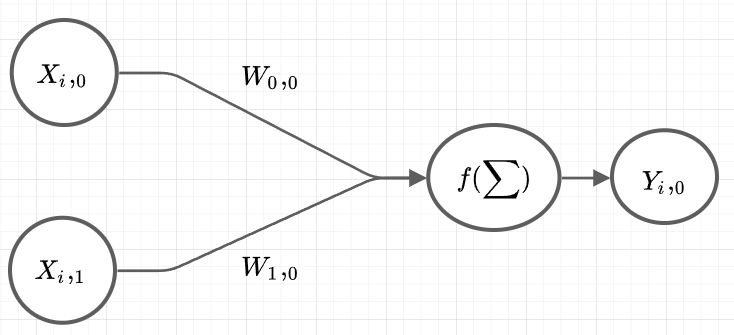
\includegraphics[width=0.5\textwidth,height=\textheight]{./img/NN_01_v4.png}

Yes it is the same, its the weighted sum of the inputs and evaluated the activation function with it to calculate the output of the scenario \(i\).

\hypertarget{forward-pass}{%
\section{Forward pass}\label{forward-pass}}

Now we create the so called \texttt{forward()} function in python:

\begin{Shaded}
\begin{Highlighting}[]
\KeywordTok{def}\NormalTok{ forward(x, w):}
  \ControlFlowTok{return}\NormalTok{( step(x }\OperatorTok{@}\NormalTok{ w) )}
\end{Highlighting}
\end{Shaded}

(Numpy provides us with the \texttt{@} symbol to make a matrix to matrix multiplication and the \texttt{.T} to transpose)

Because we want to put one dimensional matrices into the \texttt{step()} function we need to use numpy for the if-else statement:

\begin{Shaded}
\begin{Highlighting}[]
\KeywordTok{def}\NormalTok{ step(s):}
  \ControlFlowTok{return}\NormalTok{( np.where(s }\OperatorTok{\textgreater{}=}\NormalTok{ bias, }\DecValTok{1}\NormalTok{, }\DecValTok{0}\NormalTok{) )}
\end{Highlighting}
\end{Shaded}

Here an small example for the forward pass:

\begin{Shaded}
\begin{Highlighting}[]
\NormalTok{X }\OperatorTok{=}\NormalTok{ np.array([}
\NormalTok{  [}\DecValTok{0}\NormalTok{,}\DecValTok{0}\NormalTok{],}
\NormalTok{  [}\DecValTok{0}\NormalTok{,}\DecValTok{1}\NormalTok{],}
\NormalTok{  [}\DecValTok{1}\NormalTok{,}\DecValTok{0}\NormalTok{],}
\NormalTok{  [}\DecValTok{1}\NormalTok{,}\DecValTok{1}\NormalTok{],}
\NormalTok{])}
\NormalTok{W }\OperatorTok{=}\NormalTok{ np.array([}
\NormalTok{  [}\FloatTok{0.1}\NormalTok{], }
\NormalTok{  [}\FloatTok{0.2}\NormalTok{]}
\NormalTok{])}
\NormalTok{bias }\OperatorTok{=} \DecValTok{1}
\NormalTok{Y\_approx }\OperatorTok{=}\NormalTok{ forward(X, W)}
\BuiltInTok{print}\NormalTok{(Y\_approx)}
\end{Highlighting}
\end{Shaded}

\begin{verbatim}
## [[0]
##  [0]
##  [0]
##  [0]]
\end{verbatim}

And these are all the generated outputs of our NN over all scenarios. Now we need to calculate the error and adjust the weights accordingly.

\hypertarget{backward-pass}{%
\section{backward pass}\label{backward-pass}}

To adjust the weights in a single Perceptron, we need the Delta-Rule:
\[
  W(t+1) = W(t) + \Delta W(t)
\]
with
\[
  \Delta W(t) = \alpha \cdot X^{T} * (Y - \hat{Y})
\]
and \(\hat{Y}\) is the output of the NN.

\begin{Shaded}
\begin{Highlighting}[]
\KeywordTok{def}\NormalTok{ backward(W, X, Y, alpha, Y\_approx):}
    \ControlFlowTok{return}\NormalTok{(W }\OperatorTok{+}\NormalTok{ alpha }\OperatorTok{*}\NormalTok{ X.T }\OperatorTok{@}\NormalTok{ (Y }\OperatorTok{{-}}\NormalTok{ Y\_approx))}
\end{Highlighting}
\end{Shaded}

with the result of the forward pass and example data we have the following:

\begin{Shaded}
\begin{Highlighting}[]
\NormalTok{Y }\OperatorTok{=}\NormalTok{ np.array([}
\NormalTok{  [}\DecValTok{0}\NormalTok{],}
\NormalTok{  [}\DecValTok{1}\NormalTok{],}
\NormalTok{  [}\DecValTok{1}\NormalTok{],}
\NormalTok{  [}\DecValTok{1}\NormalTok{]}
\NormalTok{])}
\NormalTok{alpha }\OperatorTok{=} \FloatTok{0.01}
\NormalTok{W }\OperatorTok{=}\NormalTok{ backward(W, X, Y, alpha, Y\_approx)}
\BuiltInTok{print}\NormalTok{(W)}
\end{Highlighting}
\end{Shaded}

\begin{verbatim}
## [[0.12]
##  [0.22]]
\end{verbatim}

and this is the new weight.

\hypertarget{single-perceptron-1}{%
\section{Single Perceptron}\label{single-perceptron-1}}

Now we want to do the same process multiple times, to train the NN:

\begin{Shaded}
\begin{Highlighting}[]
\NormalTok{X }\OperatorTok{=}\NormalTok{ np.array([}
\NormalTok{  [}\DecValTok{0}\NormalTok{,}\DecValTok{0}\NormalTok{],}
\NormalTok{  [}\DecValTok{0}\NormalTok{,}\DecValTok{1}\NormalTok{],}
\NormalTok{  [}\DecValTok{1}\NormalTok{,}\DecValTok{0}\NormalTok{],}
\NormalTok{  [}\DecValTok{1}\NormalTok{,}\DecValTok{1}\NormalTok{],}
\NormalTok{])}
\NormalTok{Y }\OperatorTok{=}\NormalTok{ np.array([}
\NormalTok{  [}\DecValTok{0}\NormalTok{],}
\NormalTok{  [}\DecValTok{1}\NormalTok{],}
\NormalTok{  [}\DecValTok{1}\NormalTok{],}
\NormalTok{  [}\DecValTok{1}\NormalTok{]}
\NormalTok{])}
\NormalTok{W }\OperatorTok{=}\NormalTok{ np.array([}
\NormalTok{  [}\FloatTok{0.1}\NormalTok{], }
\NormalTok{  [}\FloatTok{0.2}\NormalTok{]}
\NormalTok{])}
\NormalTok{alpha }\OperatorTok{=} \FloatTok{0.01}
\NormalTok{bias }\OperatorTok{=} \DecValTok{1}
\NormalTok{epochs }\OperatorTok{=} \DecValTok{100}

\NormalTok{errors }\OperatorTok{=}\NormalTok{ []}
\ControlFlowTok{for}\NormalTok{ i }\KeywordTok{in} \BuiltInTok{range}\NormalTok{(epochs):}
\NormalTok{  Y\_approx }\OperatorTok{=}\NormalTok{ forward(X, W)}
\NormalTok{  errors.append(Y }\OperatorTok{{-}}\NormalTok{ Y\_approx)}
\NormalTok{  W }\OperatorTok{=}\NormalTok{ backward(W, X, Y, alpha, Y\_approx)}
\end{Highlighting}
\end{Shaded}

The KNN is trained. Now we want to look at the errors of each epoch. We want to measure the mean-square-error with the following formula:
\[
  Error_i = \frac{1}{2} \cdot \sum(Y-\hat{Y})^2
\]
or as python code:

\begin{Shaded}
\begin{Highlighting}[]
\KeywordTok{def}\NormalTok{ mean\_square\_error(error):}
  \ControlFlowTok{return}\NormalTok{( }\FloatTok{0.5} \OperatorTok{*}\NormalTok{ np.}\BuiltInTok{sum}\NormalTok{(error }\OperatorTok{**} \DecValTok{2}\NormalTok{) )}
\end{Highlighting}
\end{Shaded}

Now we need to calculate the mean-square-error for each element in the list \texttt{errors} which is made with \texttt{map()}:

\begin{Shaded}
\begin{Highlighting}[]
\NormalTok{mean\_square\_errors }\OperatorTok{=}\NormalTok{ np.array(}\BuiltInTok{list}\NormalTok{(}\BuiltInTok{map}\NormalTok{(mean\_square\_error, errors)))}
\end{Highlighting}
\end{Shaded}

To plot the errors, im using the following function:

\begin{Shaded}
\begin{Highlighting}[]
\KeywordTok{def}\NormalTok{ plot\_error(errors, title):}
\NormalTok{  x }\OperatorTok{=} \BuiltInTok{list}\NormalTok{(}\BuiltInTok{range}\NormalTok{(}\BuiltInTok{len}\NormalTok{(errors)))}
\NormalTok{  y }\OperatorTok{=}\NormalTok{ np.array(errors)}
\NormalTok{  pyplot.figure(figsize}\OperatorTok{=}\NormalTok{(}\DecValTok{6}\NormalTok{,}\DecValTok{6}\NormalTok{))}
\NormalTok{  pyplot.plot(x, y, }\StringTok{"g"}\NormalTok{, linewidth}\OperatorTok{=}\DecValTok{1}\NormalTok{)}
\NormalTok{  pyplot.xlabel(}\StringTok{"Iterations"}\NormalTok{, fontsize }\OperatorTok{=} \DecValTok{16}\NormalTok{)}
\NormalTok{  pyplot.ylabel(}\StringTok{"Mean Square Error"}\NormalTok{, fontsize }\OperatorTok{=} \DecValTok{16}\NormalTok{)}
\NormalTok{  pyplot.title(title)}
\NormalTok{  pyplot.ylim(}\OperatorTok{{-}}\FloatTok{0.01}\NormalTok{,}\BuiltInTok{max}\NormalTok{(errors)}\OperatorTok{*}\FloatTok{1.2}\NormalTok{)}
\NormalTok{  pyplot.show()}
  
  
\NormalTok{plot\_error(mean\_square\_errors, }\StringTok{"Single Perceptron"}\NormalTok{)}
\end{Highlighting}
\end{Shaded}

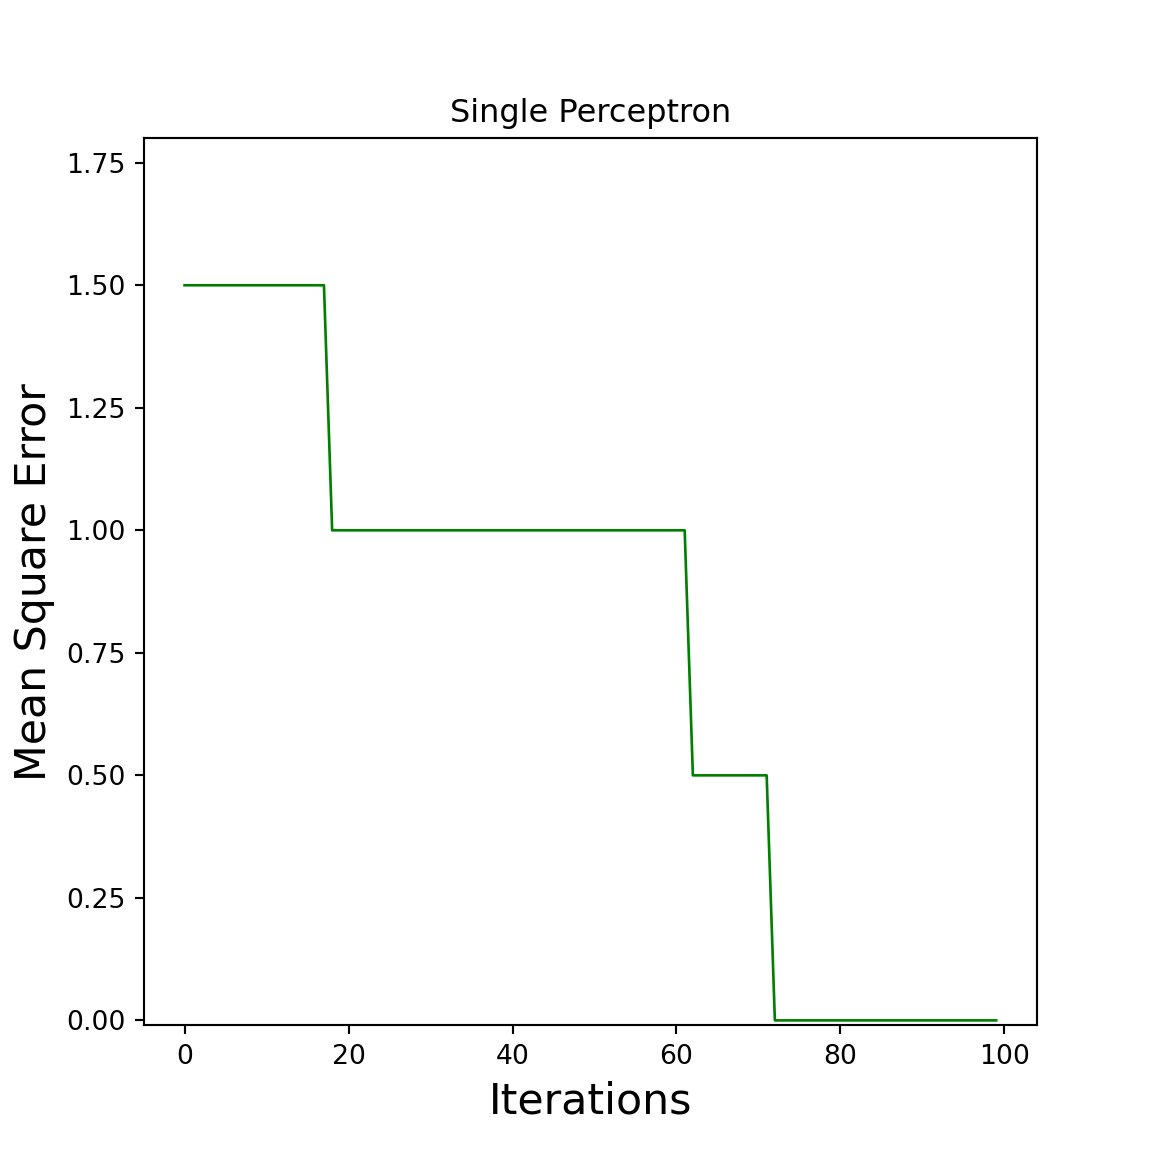
\includegraphics{gitbook-demo_files/figure-latex/0_9-1.pdf}

If you survived until now, you have learned how you can program a single Perceptron!

\hypertarget{appendix-complete-code}{%
\section{Appendix (complete code)}\label{appendix-complete-code}}

\begin{Shaded}
\begin{Highlighting}[]
\ImportTok{import}\NormalTok{ numpy }\ImportTok{as}\NormalTok{ np}
\ImportTok{import}\NormalTok{ matplotlib.pyplot }\ImportTok{as}\NormalTok{ pyplot}


\NormalTok{X }\OperatorTok{=}\NormalTok{ np.array([}
\NormalTok{  [}\DecValTok{0}\NormalTok{,}\DecValTok{0}\NormalTok{],}
\NormalTok{  [}\DecValTok{0}\NormalTok{,}\DecValTok{1}\NormalTok{],}
\NormalTok{  [}\DecValTok{1}\NormalTok{,}\DecValTok{0}\NormalTok{],}
\NormalTok{  [}\DecValTok{1}\NormalTok{,}\DecValTok{1}\NormalTok{],}
\NormalTok{])}
\NormalTok{Y }\OperatorTok{=}\NormalTok{ np.array([}
\NormalTok{  [}\DecValTok{0}\NormalTok{],}
\NormalTok{  [}\DecValTok{1}\NormalTok{],}
\NormalTok{  [}\DecValTok{1}\NormalTok{],}
\NormalTok{  [}\DecValTok{1}\NormalTok{]}
\NormalTok{])}
\NormalTok{W }\OperatorTok{=}\NormalTok{ np.array([}
\NormalTok{  [}\FloatTok{0.1}\NormalTok{], }
\NormalTok{  [}\FloatTok{0.2}\NormalTok{]}
\NormalTok{])}
\NormalTok{alpha }\OperatorTok{=} \FloatTok{0.01}
\NormalTok{bias }\OperatorTok{=} \DecValTok{1}
\NormalTok{train\_n }\OperatorTok{=} \DecValTok{100}

\KeywordTok{def}\NormalTok{ step(s):}
  \ControlFlowTok{return}\NormalTok{( np.where(s }\OperatorTok{\textgreater{}=}\NormalTok{ bias, }\DecValTok{1}\NormalTok{, }\DecValTok{0}\NormalTok{) )}


\KeywordTok{def}\NormalTok{ forward(X, W):}
  \ControlFlowTok{return}\NormalTok{( step(X }\OperatorTok{@}\NormalTok{ W) )}

\KeywordTok{def}\NormalTok{ backward(W, X, Y, alpha, Y\_approx):}
  \ControlFlowTok{return}\NormalTok{(W }\OperatorTok{+}\NormalTok{ alpha }\OperatorTok{*}\NormalTok{ X.T }\OperatorTok{@}\NormalTok{ (Y }\OperatorTok{{-}}\NormalTok{ Y\_approx))}
  
  
\NormalTok{errors }\OperatorTok{=}\NormalTok{ []}
\ControlFlowTok{for}\NormalTok{ i }\KeywordTok{in} \BuiltInTok{range}\NormalTok{(train\_n):}
\NormalTok{  Y\_approx }\OperatorTok{=}\NormalTok{ forward(X, W)}
\NormalTok{  errors.append(Y }\OperatorTok{{-}}\NormalTok{ Y\_approx)}
\NormalTok{  W }\OperatorTok{=}\NormalTok{ backward(W, X, Y, alpha, Y\_approx)}
  
  
  
\KeywordTok{def}\NormalTok{ mean\_square\_error(error):}
  \ControlFlowTok{return}\NormalTok{( }\FloatTok{0.5} \OperatorTok{*}\NormalTok{ np.}\BuiltInTok{sum}\NormalTok{(error }\OperatorTok{**} \DecValTok{2}\NormalTok{) )}


\NormalTok{mean\_square\_errors }\OperatorTok{=}\NormalTok{ np.array(}\BuiltInTok{list}\NormalTok{(}\BuiltInTok{map}\NormalTok{(mean\_square\_error, errors)))}


\KeywordTok{def}\NormalTok{ plot\_error(errors, title):}
\NormalTok{  x }\OperatorTok{=} \BuiltInTok{list}\NormalTok{(}\BuiltInTok{range}\NormalTok{(}\BuiltInTok{len}\NormalTok{(errors)))}
\NormalTok{  y }\OperatorTok{=}\NormalTok{ np.array(errors)}
\NormalTok{  pyplot.figure(figsize}\OperatorTok{=}\NormalTok{(}\DecValTok{6}\NormalTok{,}\DecValTok{6}\NormalTok{))}
\NormalTok{  pyplot.plot(x, y, }\StringTok{"g"}\NormalTok{, linewidth}\OperatorTok{=}\DecValTok{1}\NormalTok{)}
\NormalTok{  pyplot.xlabel(}\StringTok{"Iterations"}\NormalTok{, fontsize }\OperatorTok{=} \DecValTok{16}\NormalTok{)}
\NormalTok{  pyplot.ylabel(}\StringTok{"Mean Square Error"}\NormalTok{, fontsize }\OperatorTok{=} \DecValTok{16}\NormalTok{)}
\NormalTok{  pyplot.title(title)}
\NormalTok{  pyplot.ylim(}\OperatorTok{{-}}\FloatTok{0.01}\NormalTok{,}\BuiltInTok{max}\NormalTok{(errors)}\OperatorTok{*}\FloatTok{1.2}\NormalTok{)}
\NormalTok{  pyplot.show()}
  
  
\NormalTok{plot\_error(mean\_square\_errors, }\StringTok{"Single Perceptron"}\NormalTok{)}
\end{Highlighting}
\end{Shaded}

\hypertarget{adding-trainable-bias}{%
\chapter{Adding trainable Bias}\label{adding-trainable-bias}}

The single Perceptron, you saw in the previews chapter had the following activation function:
\[ 
step(s)= 
\begin{cases}
    1,& s   \geq \beta\\
    0,& s < \beta
\end{cases}
\]
with \(\beta = 1\) and that is just the right \(\beta\) for the given training dataset. But what happens if you shift the training data for example adding \(-5\) to the \(X\) matrix? Now it will never find the correct answer. That is because you need to select the \(\beta\) accordingly. But this wouldnt be intelligent to search for each dataset the optimal \(\beta\) by hand.

\hypertarget{generalising-the-bias}{%
\section{Generalising the Bias}\label{generalising-the-bias}}

That is why we now generalise the weighted sum step by step. First we generalise the activation function:
\[ 
step(s)= 
\begin{cases}
    1,& s   \geq 0\\
    0,& s < 0
\end{cases}
\]
Now we can list it in the weighted sum:
\[
  step(X * W - \beta) = Y
\]
But we have the same problem as previews, because we need to specify the \(\beta\) explicit. To add it to the training process we add a column with ones on the right side of \(X\) and add the \(-\beta\) to the last row of \(W\). The output of one scenario is now caluclated as the following:
\[
  Y_i,_0 = step([X_i,_0 \cdot W_0,_0 + X_i,_1 \cdot W_1,_0 + X_i,_2 \cdot W_2,_0]) = step([X_i,_0 \cdot W_0,_0 + X_i,_1 \cdot W_1,_0 - \beta])
\]
Furthermore because the \(W\) is holding the \(\beta\), it now gets re-adjusted in the backward pass so it is involved in the training process. Thats why we now generate a random number for it, because it gets corrected anyway.

Now we have a NN that looks like all the other pictures of a single Perceptron in the internet:\\
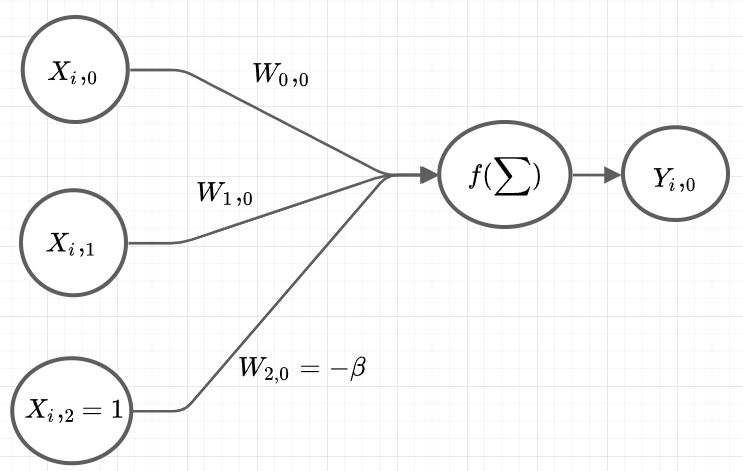
\includegraphics[width=0.5\textwidth,height=\textheight]{./img/NN_02.png}

As python code we did the following:

\begin{Shaded}
\begin{Highlighting}[]
\NormalTok{X }\OperatorTok{=}\NormalTok{ np.array([}
\NormalTok{  [}\DecValTok{0}\NormalTok{,}\DecValTok{0}\NormalTok{],}
\NormalTok{  [}\DecValTok{0}\NormalTok{,}\DecValTok{1}\NormalTok{],}
\NormalTok{  [}\DecValTok{1}\NormalTok{,}\DecValTok{0}\NormalTok{],}
\NormalTok{  [}\DecValTok{1}\NormalTok{,}\DecValTok{1}\NormalTok{],}
\NormalTok{])}\OperatorTok{{-}}\DecValTok{5}
\NormalTok{X }\OperatorTok{=}\NormalTok{ np.append(X, np.array([np.ones(}\BuiltInTok{len}\NormalTok{(X))]).T, axis}\OperatorTok{=}\DecValTok{1}\NormalTok{)}

\NormalTok{W }\OperatorTok{=}\NormalTok{ np.array([}
\NormalTok{  [}\FloatTok{0.1}\NormalTok{], }
\NormalTok{  [}\FloatTok{0.2}\NormalTok{]}
\NormalTok{])}
\NormalTok{W }\OperatorTok{=}\NormalTok{ np.append(W, }\OperatorTok{{-}}\NormalTok{np.array([np.random.random(}\BuiltInTok{len}\NormalTok{(W[}\DecValTok{0}\NormalTok{]))]).T, axis}\OperatorTok{=}\DecValTok{0}\NormalTok{)}
\end{Highlighting}
\end{Shaded}

We added \(-5\) to the \(X\) matrix to simulate the problem of shifted data, added ones on the left side of \(X\) and added negative random numbers between \((0,1)\) to the weights. Yes, if you would have a clue, what \(\beta\) would be great for the given problem, its better to choose it explicit. The new problem needs more epochs, because it needs to find a good \(\beta\) by it self.

\hypertarget{appendix-complete-code-1}{%
\section{Appendix (complete code)}\label{appendix-complete-code-1}}

The complete code is the following:

\begin{Shaded}
\begin{Highlighting}[]
\NormalTok{X }\OperatorTok{=}\NormalTok{ np.array([}
\NormalTok{  [}\DecValTok{0}\NormalTok{,}\DecValTok{0}\NormalTok{],}
\NormalTok{  [}\DecValTok{0}\NormalTok{,}\DecValTok{1}\NormalTok{],}
\NormalTok{  [}\DecValTok{1}\NormalTok{,}\DecValTok{0}\NormalTok{],}
\NormalTok{  [}\DecValTok{1}\NormalTok{,}\DecValTok{1}\NormalTok{],}
\NormalTok{]) }\OperatorTok{{-}} \DecValTok{5}
\NormalTok{X }\OperatorTok{=}\NormalTok{ np.append(X, np.array([np.ones(}\BuiltInTok{len}\NormalTok{(X))]).T, axis}\OperatorTok{=}\DecValTok{1}\NormalTok{)}

\NormalTok{W }\OperatorTok{=}\NormalTok{ np.array([}
\NormalTok{  [}\FloatTok{0.1}\NormalTok{], }
\NormalTok{  [}\FloatTok{0.2}\NormalTok{]}
\NormalTok{])}
\NormalTok{W }\OperatorTok{=}\NormalTok{ np.append(W, }\OperatorTok{{-}}\NormalTok{np.array([np.random.random(}\BuiltInTok{len}\NormalTok{(W[}\DecValTok{0}\NormalTok{]))]).T, axis}\OperatorTok{=}\DecValTok{0}\NormalTok{)}

\NormalTok{Y }\OperatorTok{=}\NormalTok{ np.array([}
\NormalTok{  [}\DecValTok{0}\NormalTok{],}
\NormalTok{  [}\DecValTok{1}\NormalTok{],}
\NormalTok{  [}\DecValTok{1}\NormalTok{],}
\NormalTok{  [}\DecValTok{1}\NormalTok{]}
\NormalTok{])}

\NormalTok{alpha }\OperatorTok{=} \FloatTok{0.01}
\NormalTok{epochs }\OperatorTok{=} \DecValTok{1000}

\KeywordTok{def}\NormalTok{ step(s):}
  \ControlFlowTok{return}\NormalTok{( np.where(s }\OperatorTok{\textgreater{}=} \DecValTok{0}\NormalTok{, }\DecValTok{1}\NormalTok{, }\DecValTok{0}\NormalTok{) )}


\KeywordTok{def}\NormalTok{ forward(X, W):}
  \ControlFlowTok{return}\NormalTok{( step(X }\OperatorTok{@}\NormalTok{ W) )}

\KeywordTok{def}\NormalTok{ backward(W, X, Y, alpha, Y\_approx):}
    \ControlFlowTok{return}\NormalTok{(W }\OperatorTok{+}\NormalTok{ alpha }\OperatorTok{*}\NormalTok{ X.T }\OperatorTok{@}\NormalTok{ (Y }\OperatorTok{{-}}\NormalTok{ Y\_approx))}
  
  
\NormalTok{errors }\OperatorTok{=}\NormalTok{ []}
\ControlFlowTok{for}\NormalTok{ i }\KeywordTok{in} \BuiltInTok{range}\NormalTok{(epochs):}
\NormalTok{  Y\_approx }\OperatorTok{=}\NormalTok{ forward(X, W)}
\NormalTok{  errors.append(Y }\OperatorTok{{-}}\NormalTok{ Y\_approx)}
\NormalTok{  W }\OperatorTok{=}\NormalTok{ backward(W, X, Y, alpha, Y\_approx)}
  
  
  
\KeywordTok{def}\NormalTok{ mean\_square\_error(error):}
  \ControlFlowTok{return}\NormalTok{( }\FloatTok{0.5} \OperatorTok{*}\NormalTok{ np.}\BuiltInTok{sum}\NormalTok{(error }\OperatorTok{**} \DecValTok{2}\NormalTok{) )}


\NormalTok{mean\_square\_errors }\OperatorTok{=}\NormalTok{ np.array(}\BuiltInTok{list}\NormalTok{(}\BuiltInTok{map}\NormalTok{(mean\_square\_error, errors)))}


\KeywordTok{def}\NormalTok{ plot\_error(errors, title):}
\NormalTok{  x }\OperatorTok{=} \BuiltInTok{list}\NormalTok{(}\BuiltInTok{range}\NormalTok{(}\BuiltInTok{len}\NormalTok{(errors)))}
\NormalTok{  y }\OperatorTok{=}\NormalTok{ np.array(errors)}
\NormalTok{  pyplot.figure(figsize}\OperatorTok{=}\NormalTok{(}\DecValTok{6}\NormalTok{,}\DecValTok{6}\NormalTok{))}
\NormalTok{  pyplot.plot(x, y, }\StringTok{"g"}\NormalTok{, linewidth}\OperatorTok{=}\DecValTok{1}\NormalTok{)}
\NormalTok{  pyplot.xlabel(}\StringTok{"Iterations"}\NormalTok{, fontsize }\OperatorTok{=} \DecValTok{16}\NormalTok{)}
\NormalTok{  pyplot.ylabel(}\StringTok{"Mean Square Error"}\NormalTok{, fontsize }\OperatorTok{=} \DecValTok{16}\NormalTok{)}
\NormalTok{  pyplot.title(title)}
\NormalTok{  pyplot.ylim(}\OperatorTok{{-}}\FloatTok{0.01}\NormalTok{,}\BuiltInTok{max}\NormalTok{(errors)}\OperatorTok{*}\FloatTok{1.2}\NormalTok{)}
\NormalTok{  pyplot.show()}
  
  
\NormalTok{plot\_error(mean\_square\_errors, }\StringTok{"Single Perceptron with trainable bias"}\NormalTok{)}
\end{Highlighting}
\end{Shaded}

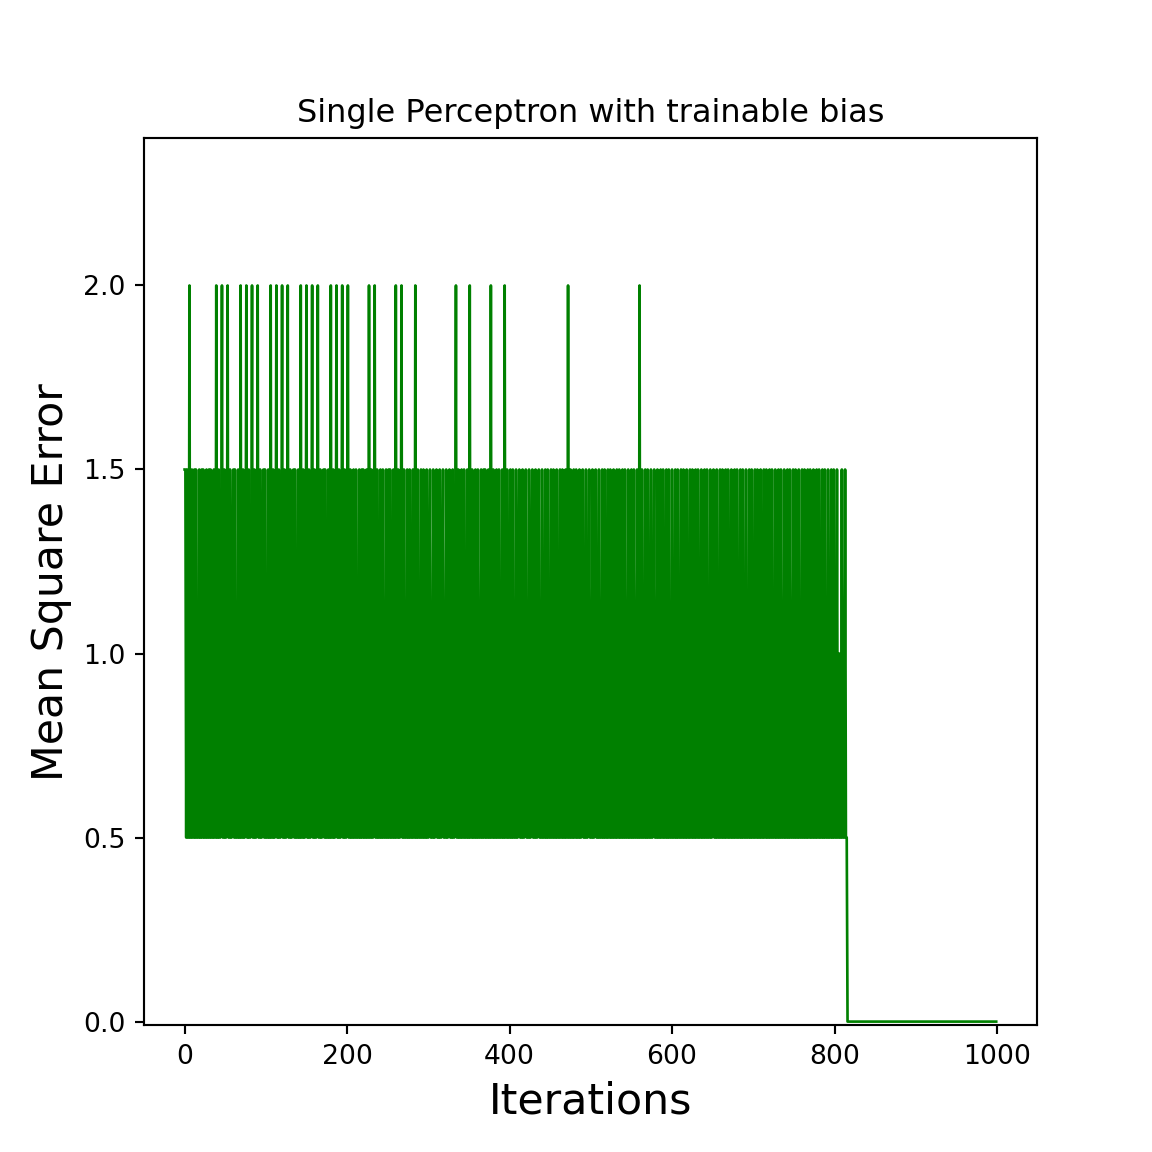
\includegraphics{gitbook-demo_files/figure-latex/1_2-3.pdf}

\hypertarget{multi-layer-perceptrons-mlp}{%
\chapter{Multi Layer Perceptrons (MLP)}\label{multi-layer-perceptrons-mlp}}

In a multi layer Perceptron you have multiple layers of neurons. Thats why we need to calculate the forward pass multiple times and the same for the backward pass. First of all, do we need to generalise some definitions, to support this behavior. What we want to do is the NN of the following picture:\\
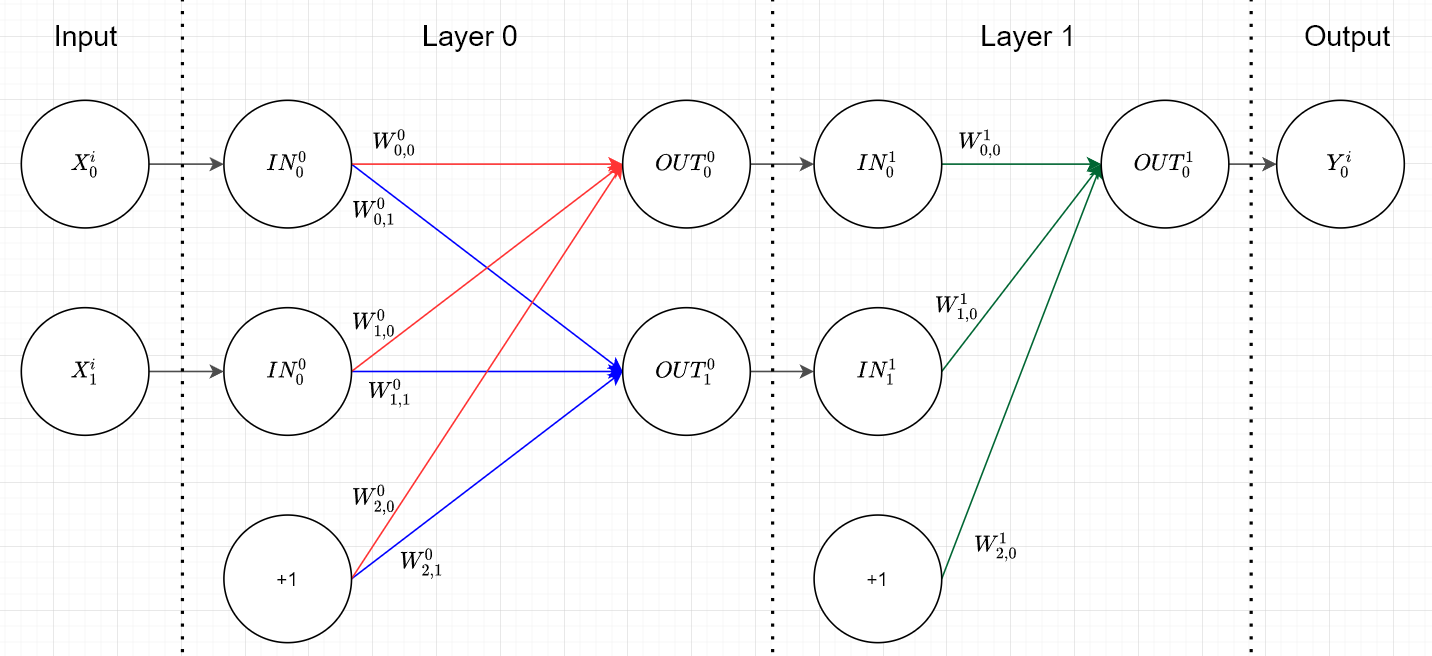
\includegraphics[width=1\textwidth,height=\textheight]{./img/NN_03_new.png}

It is my own definition of layers, because i thought, it would be better to display layers like shown in the picture, to take the step from \(n\) to \(n+1\) hidden layers more easy. You can see that each layer has the same process in the forward pass by evaluating \(f(IN^{layer} \cdot W^{layer}) = OUT^{layer}\) and just passing the result to the next layer like \(OUT^{layer} = IN^{layer+1}\), with \(f\) as the chosen activation function.\\
We will choose the sigmoid function as the activation function \(f\), because it has an easy deviation \(f^`\) for the backward pass and its very close to the behavior of the heavyside function.

\begin{Shaded}
\begin{Highlighting}[]
\KeywordTok{def}\NormalTok{ sigmoid(x):}
  \ControlFlowTok{return} \FloatTok{1.0} \OperatorTok{/}\NormalTok{ (}\FloatTok{1.0} \OperatorTok{+}\NormalTok{ np.exp(}\OperatorTok{{-}}\NormalTok{x))}

\KeywordTok{def}\NormalTok{ deriv\_sigmoid(x):}
  \ControlFlowTok{return}\NormalTok{ x }\OperatorTok{*}\NormalTok{ (}\DecValTok{1} \OperatorTok{{-}}\NormalTok{ x)}
\end{Highlighting}
\end{Shaded}

Additionaly will we choose the XOR-Gate as training dataset and generate the weights in a very generic approach like the following code shows:

\begin{Shaded}
\begin{Highlighting}[]
\NormalTok{X }\OperatorTok{=}\NormalTok{ np.array([}
\NormalTok{  [}\DecValTok{0}\NormalTok{,}\DecValTok{0}\NormalTok{],}
\NormalTok{  [}\DecValTok{0}\NormalTok{,}\DecValTok{1}\NormalTok{],}
\NormalTok{  [}\DecValTok{1}\NormalTok{,}\DecValTok{0}\NormalTok{],}
\NormalTok{  [}\DecValTok{1}\NormalTok{,}\DecValTok{1}\NormalTok{],}
\NormalTok{]) }

\NormalTok{Y }\OperatorTok{=}\NormalTok{ np.array([}
\NormalTok{  [}\DecValTok{0}\NormalTok{],}
\NormalTok{  [}\DecValTok{1}\NormalTok{],}
\NormalTok{  [}\DecValTok{1}\NormalTok{],}
\NormalTok{  [}\DecValTok{0}\NormalTok{]}
\NormalTok{])}

\NormalTok{n\_input }\OperatorTok{=} \BuiltInTok{len}\NormalTok{(X[}\DecValTok{0}\NormalTok{])}
\NormalTok{n\_output }\OperatorTok{=} \BuiltInTok{len}\NormalTok{(Y[}\DecValTok{0}\NormalTok{])}
\NormalTok{hidden\_layer\_neurons }\OperatorTok{=}\NormalTok{ np.array([}\DecValTok{2}\NormalTok{]) }\CommentTok{\# the 2 means that there is one hidden layer with 2 neurons}

\KeywordTok{def}\NormalTok{ generate\_weights(n\_input, n\_output, hidden\_layer\_neurons):}
\NormalTok{  W }\OperatorTok{=}\NormalTok{ []}
  \ControlFlowTok{for}\NormalTok{ i }\KeywordTok{in} \BuiltInTok{range}\NormalTok{(}\BuiltInTok{len}\NormalTok{(hidden\_layer\_neurons)}\OperatorTok{+}\DecValTok{1}\NormalTok{):}
    \ControlFlowTok{if}\NormalTok{ i }\OperatorTok{==} \DecValTok{0}\NormalTok{: }\CommentTok{\# first layer}
\NormalTok{      W.append(np.random.random((n\_input}\OperatorTok{+}\DecValTok{1}\NormalTok{, hidden\_layer\_neurons[i])))}
    \ControlFlowTok{elif}\NormalTok{ i }\OperatorTok{==} \BuiltInTok{len}\NormalTok{(hidden\_layer\_neurons): }\CommentTok{\# last layer}
\NormalTok{      W.append(np.random.random((hidden\_layer\_neurons[i}\OperatorTok{{-}}\DecValTok{1}\NormalTok{]}\OperatorTok{+}\DecValTok{1}\NormalTok{, n\_output)))}
    \ControlFlowTok{else}\NormalTok{: }\CommentTok{\# middle layers}
\NormalTok{      W.append(np.random.random((hidden\_layer\_neurons[i}\OperatorTok{{-}}\DecValTok{1}\NormalTok{]}\OperatorTok{+}\DecValTok{1}\NormalTok{, hidden\_layer\_neurons[i])))}
   
  \ControlFlowTok{return}\NormalTok{(W)}

\NormalTok{W }\OperatorTok{=}\NormalTok{ generate\_weights(n\_input, n\_output, hidden\_layer\_neurons)}

\BuiltInTok{print}\NormalTok{(}\StringTok{"W[0]: }\CharTok{\textbackslash{}n}\StringTok{"}\NormalTok{, W[}\DecValTok{0}\NormalTok{])}
\BuiltInTok{print}\NormalTok{(}\StringTok{"W[1]: }\CharTok{\textbackslash{}n}\StringTok{"}\NormalTok{, W[}\DecValTok{1}\NormalTok{])}
\end{Highlighting}
\end{Shaded}

\begin{verbatim}
## W[0]: 
##  [[0.64457219 0.9852289 ]
##  [0.97443724 0.60190663]
##  [0.66631054 0.10114835]]
## W[1]: 
##  [[0.88275856]
##  [0.1940694 ]
##  [0.29011425]]
\end{verbatim}

The input and output layer neurons are calculated from the training dataset and the neurons from the hidden layers are generated with the \texttt{hidden\_layer\_neurons}. For example can we generate two hidden layers with 4 and 2 neurons by \texttt{hidden\_layer\_neurons\ =\ np.array({[}4,2{]})}. I didnt explicitly choose the bias because it gets corrected anyway.\\
Now we need to define a helper function to add the biases, on the last column of the inputs, with:

\begin{Shaded}
\begin{Highlighting}[]
\KeywordTok{def}\NormalTok{ add\_ones\_to\_input(x):}
  \ControlFlowTok{return}\NormalTok{(np.append(x, np.array([np.ones(}\BuiltInTok{len}\NormalTok{(x))]).T, axis}\OperatorTok{=}\DecValTok{1}\NormalTok{))}
\end{Highlighting}
\end{Shaded}

\hypertarget{forward-pass-1}{%
\section{forward pass}\label{forward-pass-1}}

The new forward function looks exactly like in the single Perceptron:

\begin{Shaded}
\begin{Highlighting}[]
\KeywordTok{def}\NormalTok{ forward(x, w):}
  \ControlFlowTok{return}\NormalTok{( sigmoid(x }\OperatorTok{@}\NormalTok{ w) )}
\end{Highlighting}
\end{Shaded}

Now we have everything to calculate the forward pass of the NN from above with the generated weights step by step:

\begin{Shaded}
\begin{Highlighting}[]
\NormalTok{IN }\OperatorTok{=}\NormalTok{ []}
\NormalTok{OUT }\OperatorTok{=}\NormalTok{ []}

\CommentTok{\# layer 0}
\NormalTok{i }\OperatorTok{=} \DecValTok{0}
\NormalTok{IN.append( add\_ones\_to\_input(X) )}
\NormalTok{OUT.append( forward(IN[i], W[i]) )}

\CommentTok{\# layer 1}
\NormalTok{i }\OperatorTok{=} \DecValTok{1}
\NormalTok{IN.append( add\_ones\_to\_input(OUT[i}\OperatorTok{{-}}\DecValTok{1}\NormalTok{]) )}
\NormalTok{OUT.append( forward(IN[i], W[i]) )}

\CommentTok{\# error}
\NormalTok{Y}\OperatorTok{{-}}\NormalTok{OUT[}\OperatorTok{{-}}\DecValTok{1}\NormalTok{]}
\end{Highlighting}
\end{Shaded}

\begin{verbatim}
## array([[-0.72616869],
##        [ 0.23878516],
##        [ 0.24406255],
##        [-0.77818969]])
\end{verbatim}

Thats all! We calculated the forward pass in a very generic way for the NN with 2 input neurons, 2 hidden neurons and 1 output neuron for all 4 scenarios at the same time. Sadly is the forward pass the easiest part of the multi layer Perceptron :)

\hypertarget{backward-pass-1}{%
\section{backward pass}\label{backward-pass-1}}

We will adjust the weights with the backpropagation algorithm what is a special case of the descent gradient algorithm. In the output layer is it done by calculating the sensitives of the outputs according to the activation function multiplied with the error that occured. On all other layers its calculated by passing backwards the earlier calculated gradient splitted up on each neuron by the previes weights and multiplied by the sensitivity of the outputs of that layer according to the activation function. The formula is the following:
\[
  grad^i= 
\begin{cases}
    f^`(OUT^i) \cdot (Y-OUT^i),& i =\text{last layer}\\
    f^`(OUT^i) \cdot (grad^{i+1} * \widetilde{W}^{i+1\ T}),& \text{else}
\end{cases}
\]
with \(\widetilde{W}\) as the weights of that layer without the connection to the bias neuron, because it has no connection to the previews neurons. In our datastructur its done by removing the last row.\\
With the example from above is it done by the following lines of code:

\begin{Shaded}
\begin{Highlighting}[]
\NormalTok{grad }\OperatorTok{=}\NormalTok{ [}\VariableTok{None}\NormalTok{] }\OperatorTok{*} \DecValTok{2}

\CommentTok{\# layer 1}
\NormalTok{i }\OperatorTok{=} \DecValTok{1}
\NormalTok{grad[i] }\OperatorTok{=}\NormalTok{ deriv\_sigmoid(OUT[i]) }\OperatorTok{*}\NormalTok{ (Y}\OperatorTok{{-}}\NormalTok{OUT[i])}

\CommentTok{\# layer 0}
\NormalTok{i }\OperatorTok{=} \DecValTok{0}
\NormalTok{grad[i] }\OperatorTok{=}\NormalTok{ deriv\_sigmoid(OUT[i]) }\OperatorTok{*}\NormalTok{(grad[i}\OperatorTok{+}\DecValTok{1}\NormalTok{] }\OperatorTok{@}\NormalTok{ W[i}\OperatorTok{+}\DecValTok{1}\NormalTok{][}\DecValTok{0}\NormalTok{:}\BuiltInTok{len}\NormalTok{(W[i}\OperatorTok{+}\DecValTok{1}\NormalTok{])}\OperatorTok{{-}}\DecValTok{1}\NormalTok{].T) }\CommentTok{\# without bias weights}
\end{Highlighting}
\end{Shaded}

Now you can look for example at the gradient of the last layer and on the direction it is shown:

\begin{Shaded}
\begin{Highlighting}[]
\BuiltInTok{print}\NormalTok{(}\StringTok{"Y: }\CharTok{\textbackslash{}n}\StringTok{"}\NormalTok{,Y)}
\BuiltInTok{print}\NormalTok{(}\StringTok{"OUT: }\CharTok{\textbackslash{}n}\StringTok{"}\NormalTok{,OUT[}\DecValTok{1}\NormalTok{])}
\BuiltInTok{print}\NormalTok{(}\StringTok{"grad: }\CharTok{\textbackslash{}n}\StringTok{"}\NormalTok{,grad[}\DecValTok{1}\NormalTok{])}
\end{Highlighting}
\end{Shaded}

\begin{verbatim}
## Y: 
##  [[0]
##  [1]
##  [1]
##  [0]]
## OUT: 
##  [[0.72616869]
##  [0.76121484]
##  [0.75593745]
##  [0.77818969]]
## grad: 
##  [[-0.14439699]
##  [ 0.04340322]
##  [ 0.04502857]
##  [-0.13432371]]
\end{verbatim}

You can see that the gradient shows in the direction that would drift the output \(OUT\) closer to the desired output \(Y\). That is exactly what the gradient descent algorithm is doing.\\
Now do we need to adjust the weights with the gradients and the learningrate \(\alpha\) according to the direction of the gradients with the following formula:
\[
  W^i_{new} = W^i_{old} + \alpha \cdot ( IN^{i\ T} * grad^i) 
\]
In the example from above we have the following results for the adjusted weights after the first iteration:

\begin{Shaded}
\begin{Highlighting}[]
\NormalTok{alpha }\OperatorTok{=} \FloatTok{0.03}

\NormalTok{W[}\DecValTok{1}\NormalTok{] }\OperatorTok{=}\NormalTok{ W[}\DecValTok{1}\NormalTok{] }\OperatorTok{+}\NormalTok{ alpha }\OperatorTok{*}\NormalTok{ (IN[}\DecValTok{1}\NormalTok{].T }\OperatorTok{@}\NormalTok{ grad[}\DecValTok{1}\NormalTok{]) }
\NormalTok{W[}\DecValTok{0}\NormalTok{] }\OperatorTok{=}\NormalTok{ W[}\DecValTok{0}\NormalTok{] }\OperatorTok{+}\NormalTok{ alpha }\OperatorTok{*}\NormalTok{ (IN[}\DecValTok{0}\NormalTok{].T }\OperatorTok{@}\NormalTok{ grad[}\DecValTok{0}\NormalTok{]) }
\end{Highlighting}
\end{Shaded}

This was the process of the forward pass and backward pass for one epoch in the multi layer Perceptron with 2 input neurons 2 hidden layer neurons an done output neuron. It is simple to use the given code from above to create a more generic NN for dynamic hidden layers and with dynamic training datasets for the given amount of epochs like in the appendix below.

\hypertarget{appendix-complete-code-2}{%
\section{Appendix (complete code)}\label{appendix-complete-code-2}}

\begin{Shaded}
\begin{Highlighting}[]
\ImportTok{import}\NormalTok{ numpy }\ImportTok{as}\NormalTok{ np}
\ImportTok{import}\NormalTok{ matplotlib.pyplot }\ImportTok{as}\NormalTok{ pyplot}
\NormalTok{np.random.seed(}\DecValTok{0}\NormalTok{)}

\NormalTok{X }\OperatorTok{=}\NormalTok{ np.array([}
\NormalTok{  [}\DecValTok{1}\NormalTok{,}\DecValTok{1}\NormalTok{],}
\NormalTok{  [}\DecValTok{0}\NormalTok{,}\DecValTok{1}\NormalTok{],}
\NormalTok{  [}\DecValTok{1}\NormalTok{,}\DecValTok{0}\NormalTok{],}
\NormalTok{  [}\DecValTok{0}\NormalTok{,}\DecValTok{0}\NormalTok{],}
\NormalTok{])}

\NormalTok{Y }\OperatorTok{=}\NormalTok{ np.array([}
\NormalTok{  [}\DecValTok{0}\NormalTok{],}
\NormalTok{  [}\DecValTok{1}\NormalTok{],}
\NormalTok{  [}\DecValTok{1}\NormalTok{],}
\NormalTok{  [}\DecValTok{0}\NormalTok{]}
\NormalTok{])}

\NormalTok{n\_input }\OperatorTok{=} \BuiltInTok{len}\NormalTok{(X[}\DecValTok{0}\NormalTok{])}
\NormalTok{n\_output }\OperatorTok{=} \BuiltInTok{len}\NormalTok{(Y[}\DecValTok{0}\NormalTok{])}
\NormalTok{hidden\_layer\_neurons }\OperatorTok{=}\NormalTok{ np.array([}\DecValTok{2}\NormalTok{])}


\KeywordTok{def}\NormalTok{ generate\_weights(n\_input, n\_output, hidden\_layer\_neurons):}
\NormalTok{  W }\OperatorTok{=}\NormalTok{ []}
  \ControlFlowTok{for}\NormalTok{ i }\KeywordTok{in} \BuiltInTok{range}\NormalTok{(}\BuiltInTok{len}\NormalTok{(hidden\_layer\_neurons)}\OperatorTok{+}\DecValTok{1}\NormalTok{):}
    \ControlFlowTok{if}\NormalTok{ i }\OperatorTok{==} \DecValTok{0}\NormalTok{: }\CommentTok{\# first layer}
\NormalTok{      W.append(np.random.random((n\_input }\OperatorTok{+} \DecValTok{1}\NormalTok{, hidden\_layer\_neurons[i])))}
    \ControlFlowTok{elif}\NormalTok{ i }\OperatorTok{==} \BuiltInTok{len}\NormalTok{(hidden\_layer\_neurons): }\CommentTok{\# last layer}
\NormalTok{      W.append(np.random.random((hidden\_layer\_neurons[i}\OperatorTok{{-}}\DecValTok{1}\NormalTok{]}\OperatorTok{+}\DecValTok{1}\NormalTok{, n\_output)))}
    \ControlFlowTok{else}\NormalTok{: }\CommentTok{\# middle layers}
\NormalTok{      W.append(np.random.random((hidden\_layer\_neurons[i}\OperatorTok{{-}}\DecValTok{1}\NormalTok{]}\OperatorTok{+}\DecValTok{1}\NormalTok{, hidden\_layer\_neurons[i])))}
  \ControlFlowTok{return}\NormalTok{(W)}

\KeywordTok{def}\NormalTok{ add\_ones\_to\_input(x):}
  \ControlFlowTok{return}\NormalTok{(np.append(x, np.array([np.ones(}\BuiltInTok{len}\NormalTok{(x))]).T, axis}\OperatorTok{=}\DecValTok{1}\NormalTok{))}


\NormalTok{W }\OperatorTok{=}\NormalTok{ generate\_weights(n\_input, n\_output, hidden\_layer\_neurons)}


\KeywordTok{def}\NormalTok{ sigmoid(x):}
  \ControlFlowTok{return} \FloatTok{1.0} \OperatorTok{/}\NormalTok{ (}\FloatTok{1.0} \OperatorTok{+}\NormalTok{ np.exp(}\OperatorTok{{-}}\NormalTok{x))}

\KeywordTok{def}\NormalTok{ deriv\_sigmoid(x):}
  \ControlFlowTok{return}\NormalTok{ x }\OperatorTok{*}\NormalTok{ (}\DecValTok{1} \OperatorTok{{-}}\NormalTok{ x)}


\KeywordTok{def}\NormalTok{ forward(x, w):}
  \ControlFlowTok{return}\NormalTok{( sigmoid(x }\OperatorTok{@}\NormalTok{ w) )}

\KeywordTok{def}\NormalTok{ backward(IN, OUT, W, Y, grad, k):}
  \ControlFlowTok{if}\NormalTok{ k }\OperatorTok{==} \BuiltInTok{len}\NormalTok{(grad)}\OperatorTok{{-}}\DecValTok{1}\NormalTok{:}
\NormalTok{    grad[k] }\OperatorTok{=}\NormalTok{ deriv\_sigmoid(OUT[k]) }\OperatorTok{*}\NormalTok{ (Y}\OperatorTok{{-}}\NormalTok{OUT[k])}
  \ControlFlowTok{else}\NormalTok{:}
\NormalTok{    grad[k] }\OperatorTok{=}\NormalTok{ deriv\_sigmoid(OUT[k]) }\OperatorTok{*}\NormalTok{(grad[k}\OperatorTok{+}\DecValTok{1}\NormalTok{] }\OperatorTok{@}\NormalTok{ W[k}\OperatorTok{+}\DecValTok{1}\NormalTok{][}\DecValTok{0}\NormalTok{:}\BuiltInTok{len}\NormalTok{(W[k}\OperatorTok{+}\DecValTok{1}\NormalTok{])}\OperatorTok{{-}}\DecValTok{1}\NormalTok{].T)}
  \ControlFlowTok{return}\NormalTok{(grad)}

\NormalTok{alpha }\OperatorTok{=} \FloatTok{0.03}
\NormalTok{errors }\OperatorTok{=}\NormalTok{ []}
\ControlFlowTok{for}\NormalTok{ i }\KeywordTok{in} \BuiltInTok{range}\NormalTok{(}\DecValTok{40000}\NormalTok{):}
\NormalTok{  IN }\OperatorTok{=}\NormalTok{ []}
\NormalTok{  OUT }\OperatorTok{=}\NormalTok{ []}
\NormalTok{  grad }\OperatorTok{=}\NormalTok{ [}\VariableTok{None}\NormalTok{]}\OperatorTok{*}\BuiltInTok{len}\NormalTok{(W)}
  \ControlFlowTok{for}\NormalTok{ k }\KeywordTok{in} \BuiltInTok{range}\NormalTok{(}\BuiltInTok{len}\NormalTok{(W)):}
    \ControlFlowTok{if}\NormalTok{ k}\OperatorTok{==}\DecValTok{0}\NormalTok{:}
\NormalTok{      IN.append(add\_ones\_to\_input(X))}
    \ControlFlowTok{else}\NormalTok{:}
\NormalTok{      IN.append(add\_ones\_to\_input(OUT[k}\OperatorTok{{-}}\DecValTok{1}\NormalTok{]))}
\NormalTok{    OUT.append(forward(x}\OperatorTok{=}\NormalTok{IN[k], w}\OperatorTok{=}\NormalTok{W[k]))}
    
\NormalTok{  errors.append(Y }\OperatorTok{{-}}\NormalTok{ OUT[}\OperatorTok{{-}}\DecValTok{1}\NormalTok{])}
    
  \ControlFlowTok{for}\NormalTok{ k }\KeywordTok{in} \BuiltInTok{range}\NormalTok{(}\BuiltInTok{len}\NormalTok{(W)}\OperatorTok{{-}}\DecValTok{1}\NormalTok{,}\OperatorTok{{-}}\DecValTok{1}\NormalTok{, }\OperatorTok{{-}}\DecValTok{1}\NormalTok{):}
\NormalTok{    grad }\OperatorTok{=}\NormalTok{ backward(IN, OUT, W, Y, grad, k) }
    
  \ControlFlowTok{for}\NormalTok{ k }\KeywordTok{in} \BuiltInTok{range}\NormalTok{(}\BuiltInTok{len}\NormalTok{(W)):}
\NormalTok{    W[k] }\OperatorTok{=}\NormalTok{ W[k] }\OperatorTok{+}\NormalTok{ alpha }\OperatorTok{*}\NormalTok{ (IN[k].T }\OperatorTok{@}\NormalTok{ grad[k])}



\KeywordTok{def}\NormalTok{ mean\_square\_error(error):}
  \ControlFlowTok{return}\NormalTok{( }\FloatTok{0.5} \OperatorTok{*}\NormalTok{ np.}\BuiltInTok{sum}\NormalTok{(error }\OperatorTok{**} \DecValTok{2}\NormalTok{) )}

\NormalTok{mean\_square\_errors }\OperatorTok{=}\NormalTok{ np.array(}\BuiltInTok{list}\NormalTok{(}\BuiltInTok{map}\NormalTok{(mean\_square\_error, errors)))}

\KeywordTok{def}\NormalTok{ plot\_error(errors, title):}
\NormalTok{  x }\OperatorTok{=} \BuiltInTok{list}\NormalTok{(}\BuiltInTok{range}\NormalTok{(}\BuiltInTok{len}\NormalTok{(errors)))}
\NormalTok{  y }\OperatorTok{=}\NormalTok{ np.array(errors)}
\NormalTok{  pyplot.figure(figsize}\OperatorTok{=}\NormalTok{(}\DecValTok{6}\NormalTok{,}\DecValTok{6}\NormalTok{))}
\NormalTok{  pyplot.plot(x, y, }\StringTok{"g"}\NormalTok{, linewidth}\OperatorTok{=}\DecValTok{1}\NormalTok{)}
\NormalTok{  pyplot.xlabel(}\StringTok{"Iterations"}\NormalTok{, fontsize }\OperatorTok{=} \DecValTok{16}\NormalTok{)}
\NormalTok{  pyplot.ylabel(}\StringTok{"Mean Square Error"}\NormalTok{, fontsize }\OperatorTok{=} \DecValTok{16}\NormalTok{)}
\NormalTok{  pyplot.title(title)}
\NormalTok{  pyplot.ylim(}\DecValTok{0}\NormalTok{,}\DecValTok{1}\NormalTok{)}
\NormalTok{  pyplot.show()}
  
\NormalTok{plot\_error(mean\_square\_errors, }\StringTok{"Mean{-}Square{-}Errors of MLP 2x2x1"}\NormalTok{)}
\end{Highlighting}
\end{Shaded}

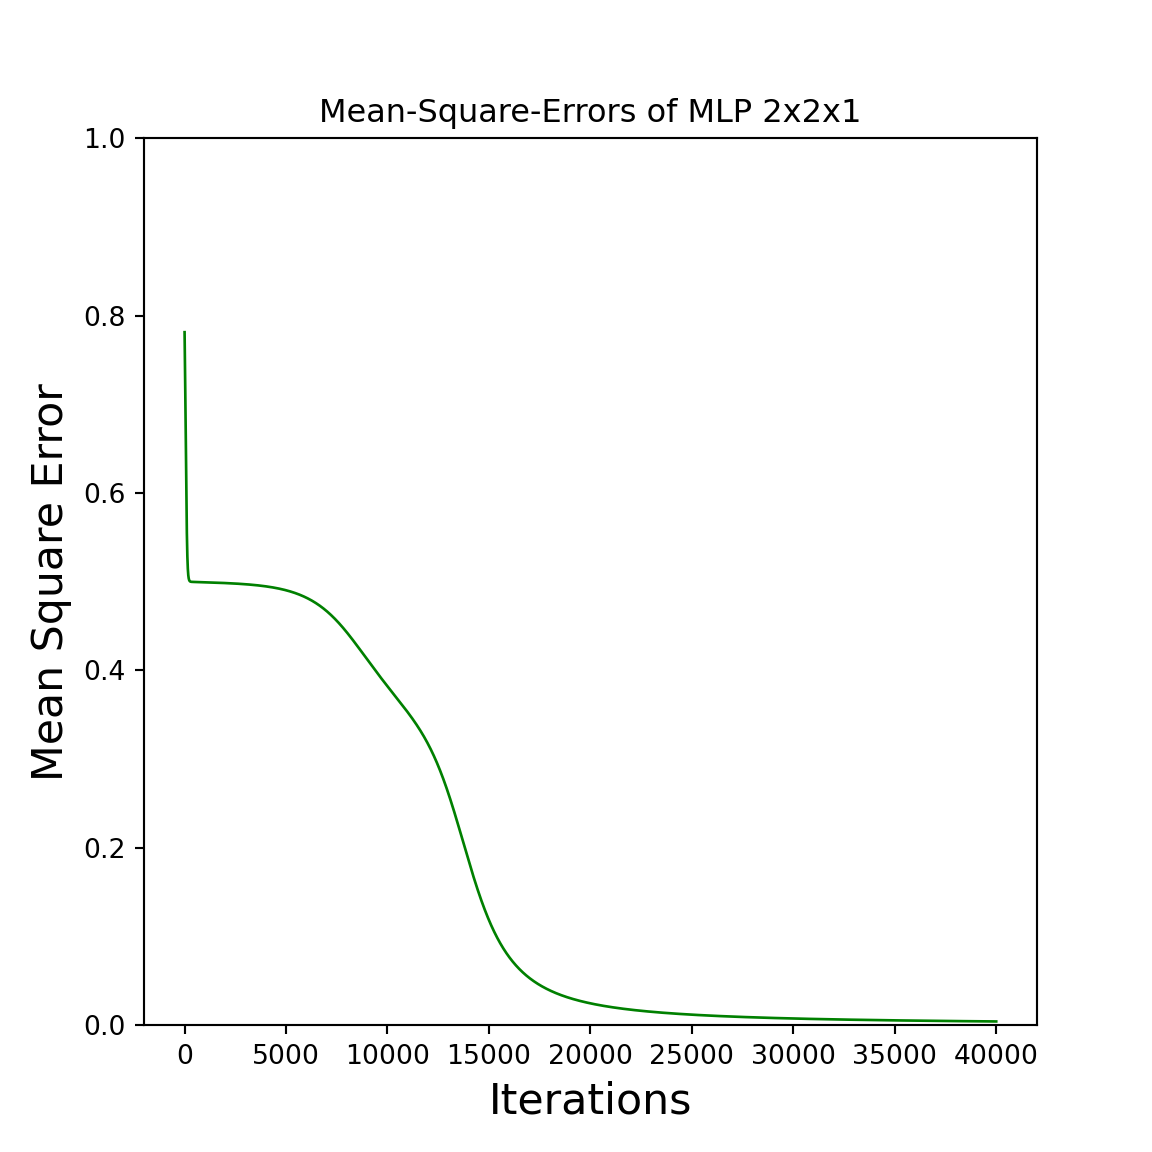
\includegraphics{gitbook-demo_files/figure-latex/2_9-5.pdf}

\hypertarget{mlp-example-credit-default}{%
\chapter{MLP example (Credit Default)}\label{mlp-example-credit-default}}

Now can we use our generic MLP model from the previews chapter to forecast real life credit defaults. The csv can be downloaded from \href{https://www.kaggle.com/laotse/credit-risk-dataset}{Kaggle Data Source} or from my \href{https://github.com/AxelCode-R/GitBook}{github repo} in the example\_data folder.

\hypertarget{appendix-complete-code-3}{%
\section{Appendix (complete code)}\label{appendix-complete-code-3}}

\begin{Shaded}
\begin{Highlighting}[]
\ImportTok{import}\NormalTok{ numpy }\ImportTok{as}\NormalTok{ np}
\ImportTok{import}\NormalTok{ matplotlib.pyplot }\ImportTok{as}\NormalTok{ pyplot}
\ImportTok{import}\NormalTok{ pandas }\ImportTok{as}\NormalTok{ pd}
\ImportTok{from}\NormalTok{ sklearn.metrics }\ImportTok{import}\NormalTok{ confusion\_matrix}
\NormalTok{np.random.seed(}\DecValTok{0}\NormalTok{)}

\NormalTok{data }\OperatorTok{=}\NormalTok{ pd.read\_csv(}\StringTok{"example\_data/credit\_risk\_dataset.csv"}\NormalTok{).fillna(}\DecValTok{0}\NormalTok{)}
\NormalTok{data }\OperatorTok{=}\NormalTok{ data.replace(\{}\StringTok{"Y"}\NormalTok{: }\DecValTok{1}\NormalTok{, }\StringTok{"N"}\NormalTok{:}\DecValTok{0}\NormalTok{\})}

\NormalTok{scale\_mapper }\OperatorTok{=}\NormalTok{ \{}\StringTok{\textquotesingle{}OWN\textquotesingle{}}\NormalTok{:}\DecValTok{1}\NormalTok{, }\StringTok{\textquotesingle{}RENT\textquotesingle{}}\NormalTok{:}\DecValTok{2}\NormalTok{, }\StringTok{\textquotesingle{}MORTGAGE\textquotesingle{}}\NormalTok{:}\DecValTok{3}\NormalTok{, }\StringTok{\textquotesingle{}OTHER\textquotesingle{}}\NormalTok{:}\DecValTok{4}\NormalTok{\}}
\NormalTok{data[}\StringTok{"person\_home\_ownership"}\NormalTok{] }\OperatorTok{=}\NormalTok{ data[}\StringTok{"person\_home\_ownership"}\NormalTok{].replace(scale\_mapper)}
\NormalTok{scale\_mapper }\OperatorTok{=}\NormalTok{ \{}\StringTok{\textquotesingle{}PERSONAL\textquotesingle{}}\NormalTok{:}\DecValTok{1}\NormalTok{, }\StringTok{\textquotesingle{}EDUCATION\textquotesingle{}}\NormalTok{:}\DecValTok{2}\NormalTok{, }\StringTok{\textquotesingle{}MEDICAL\textquotesingle{}}\NormalTok{:}\DecValTok{3}\NormalTok{, }\StringTok{\textquotesingle{}VENTURE\textquotesingle{}}\NormalTok{:}\DecValTok{4}\NormalTok{, }\StringTok{\textquotesingle{}HOMEIMPROVEMENT\textquotesingle{}}\NormalTok{:}\DecValTok{5}\NormalTok{,}\StringTok{\textquotesingle{}DEBTCONSOLIDATION\textquotesingle{}}\NormalTok{:}\DecValTok{6}\NormalTok{\}}
\NormalTok{data[}\StringTok{"loan\_intent"}\NormalTok{] }\OperatorTok{=}\NormalTok{ data[}\StringTok{"loan\_intent"}\NormalTok{].replace(scale\_mapper)}
\NormalTok{scale\_mapper }\OperatorTok{=}\NormalTok{ \{}\StringTok{\textquotesingle{}A\textquotesingle{}}\NormalTok{:}\DecValTok{1}\NormalTok{, }\StringTok{\textquotesingle{}B\textquotesingle{}}\NormalTok{:}\DecValTok{2}\NormalTok{, }\StringTok{\textquotesingle{}C\textquotesingle{}}\NormalTok{:}\DecValTok{3}\NormalTok{, }\StringTok{\textquotesingle{}D\textquotesingle{}}\NormalTok{:}\DecValTok{4}\NormalTok{, }\StringTok{\textquotesingle{}E\textquotesingle{}}\NormalTok{:}\DecValTok{5}\NormalTok{, }\StringTok{\textquotesingle{}F\textquotesingle{}}\NormalTok{:}\DecValTok{6}\NormalTok{, }\StringTok{\textquotesingle{}G\textquotesingle{}}\NormalTok{:}\DecValTok{7}\NormalTok{\}}
\NormalTok{data[}\StringTok{"loan\_grade"}\NormalTok{] }\OperatorTok{=}\NormalTok{ data[}\StringTok{"loan\_grade"}\NormalTok{].replace(scale\_mapper)}


\KeywordTok{def}\NormalTok{ NormalizeData(np\_arr):}
  \ControlFlowTok{for}\NormalTok{ i }\KeywordTok{in} \BuiltInTok{range}\NormalTok{(np\_arr.shape[}\DecValTok{1}\NormalTok{]):}
\NormalTok{    np\_arr[:,i] }\OperatorTok{=}\NormalTok{ (np\_arr[:,i] }\OperatorTok{{-}}\NormalTok{ np.}\BuiltInTok{min}\NormalTok{(np\_arr[:,i])) }\OperatorTok{/}\NormalTok{ (np.}\BuiltInTok{max}\NormalTok{(np\_arr[:,i]) }\OperatorTok{{-}}\NormalTok{ np.}\BuiltInTok{min}\NormalTok{(np\_arr[:,i]))}
  \ControlFlowTok{return}\NormalTok{(np\_arr)}

\NormalTok{training\_n }\OperatorTok{=} \DecValTok{2000}
\NormalTok{X\_train }\OperatorTok{=}\NormalTok{ NormalizeData( data.loc[}\DecValTok{0}\NormalTok{:(training\_n}\OperatorTok{{-}}\DecValTok{1}\NormalTok{), data.columns }\OperatorTok{!=} \StringTok{\textquotesingle{}loan\_status\textquotesingle{}}\NormalTok{].to\_numpy() )}
\NormalTok{Y\_train }\OperatorTok{=}\NormalTok{ data.loc[}\DecValTok{0}\NormalTok{:(training\_n}\OperatorTok{{-}}\DecValTok{1}\NormalTok{), data.columns }\OperatorTok{==} \StringTok{\textquotesingle{}loan\_status\textquotesingle{}}\NormalTok{].to\_numpy()}

\NormalTok{X\_test }\OperatorTok{=}\NormalTok{ NormalizeData( data.loc[training\_n:, data.columns }\OperatorTok{!=} \StringTok{\textquotesingle{}loan\_status\textquotesingle{}}\NormalTok{].to\_numpy() )}
\NormalTok{Y\_test }\OperatorTok{=}\NormalTok{ data.loc[training\_n:, data.columns }\OperatorTok{==} \StringTok{\textquotesingle{}loan\_status\textquotesingle{}}\NormalTok{].to\_numpy()}



\KeywordTok{def}\NormalTok{ generate\_weights(n\_input, n\_output, hidden\_layer\_neurons):}
\NormalTok{  W }\OperatorTok{=}\NormalTok{ []}
  \ControlFlowTok{for}\NormalTok{ i }\KeywordTok{in} \BuiltInTok{range}\NormalTok{(}\BuiltInTok{len}\NormalTok{(hidden\_layer\_neurons)}\OperatorTok{+}\DecValTok{1}\NormalTok{):}
    \ControlFlowTok{if}\NormalTok{ i }\OperatorTok{==} \DecValTok{0}\NormalTok{: }\CommentTok{\# first layer}
\NormalTok{      W.append(np.random.random((n\_input}\OperatorTok{+}\DecValTok{1}\NormalTok{, hidden\_layer\_neurons[i])))}
    \ControlFlowTok{elif}\NormalTok{ i }\OperatorTok{==} \BuiltInTok{len}\NormalTok{(hidden\_layer\_neurons): }\CommentTok{\# last layer}
\NormalTok{      W.append(np.random.random((hidden\_layer\_neurons[i}\OperatorTok{{-}}\DecValTok{1}\NormalTok{]}\OperatorTok{+}\DecValTok{1}\NormalTok{, n\_output)))}
    \ControlFlowTok{else}\NormalTok{: }\CommentTok{\# middle layers}
\NormalTok{      W.append(np.random.random((hidden\_layer\_neurons[i}\OperatorTok{{-}}\DecValTok{1}\NormalTok{]}\OperatorTok{+}\DecValTok{1}\NormalTok{, hidden\_layer\_neurons[i])))}
  \ControlFlowTok{return}\NormalTok{(W)}

\KeywordTok{def}\NormalTok{ add\_ones\_to\_input(x):}
  \ControlFlowTok{return}\NormalTok{(np.append(x, np.array([np.ones(}\BuiltInTok{len}\NormalTok{(x))]).T, axis}\OperatorTok{=}\DecValTok{1}\NormalTok{))}



\KeywordTok{def}\NormalTok{ sigmoid(x):}
  \ControlFlowTok{return} \FloatTok{1.0} \OperatorTok{/}\NormalTok{ (}\FloatTok{1.0} \OperatorTok{+}\NormalTok{ np.exp(}\OperatorTok{{-}}\NormalTok{x))}

\KeywordTok{def}\NormalTok{ deriv\_sigmoid(x):}
  \ControlFlowTok{return}\NormalTok{ x }\OperatorTok{*}\NormalTok{ (}\DecValTok{1} \OperatorTok{{-}}\NormalTok{ x)}


\KeywordTok{def}\NormalTok{ forward(x, w):}
  \ControlFlowTok{return}\NormalTok{( sigmoid(x }\OperatorTok{@}\NormalTok{ w) )}

\KeywordTok{def}\NormalTok{ backward(IN, OUT, W, Y, grad, k):}
  \ControlFlowTok{if}\NormalTok{ k }\OperatorTok{==} \BuiltInTok{len}\NormalTok{(grad)}\OperatorTok{{-}}\DecValTok{1}\NormalTok{:}
\NormalTok{    grad[k] }\OperatorTok{=}\NormalTok{ deriv\_sigmoid(OUT[k]) }\OperatorTok{*}\NormalTok{ (Y}\OperatorTok{{-}}\NormalTok{OUT[k])}
  \ControlFlowTok{else}\NormalTok{:}
\NormalTok{    grad[k] }\OperatorTok{=}\NormalTok{ deriv\_sigmoid(OUT[k]) }\OperatorTok{*}\NormalTok{(grad[k}\OperatorTok{+}\DecValTok{1}\NormalTok{] }\OperatorTok{@}\NormalTok{ W[k}\OperatorTok{+}\DecValTok{1}\NormalTok{][}\DecValTok{0}\NormalTok{:}\BuiltInTok{len}\NormalTok{(W[k}\OperatorTok{+}\DecValTok{1}\NormalTok{])}\OperatorTok{{-}}\DecValTok{1}\NormalTok{].T)}
  \ControlFlowTok{return}\NormalTok{(grad)}

\KeywordTok{def}\NormalTok{ train(X, Y, hidden\_layer\_neurons, alpha, epochs):}
\NormalTok{  n\_input }\OperatorTok{=} \BuiltInTok{len}\NormalTok{(X\_train[}\DecValTok{0}\NormalTok{])}
\NormalTok{  n\_output }\OperatorTok{=} \BuiltInTok{len}\NormalTok{(Y\_train[}\DecValTok{0}\NormalTok{])}
\NormalTok{  W }\OperatorTok{=}\NormalTok{ generate\_weights(n\_input, n\_output, hidden\_layer\_neurons)}
\NormalTok{  errors }\OperatorTok{=}\NormalTok{ []}
  \ControlFlowTok{for}\NormalTok{ i }\KeywordTok{in} \BuiltInTok{range}\NormalTok{(epochs):}
\NormalTok{    IN }\OperatorTok{=}\NormalTok{ []}
\NormalTok{    OUT }\OperatorTok{=}\NormalTok{ []}
\NormalTok{    grad }\OperatorTok{=}\NormalTok{ [}\VariableTok{None}\NormalTok{]}\OperatorTok{*}\BuiltInTok{len}\NormalTok{(W)}
    \ControlFlowTok{for}\NormalTok{ k }\KeywordTok{in} \BuiltInTok{range}\NormalTok{(}\BuiltInTok{len}\NormalTok{(W)):}
      \ControlFlowTok{if}\NormalTok{ k}\OperatorTok{==}\DecValTok{0}\NormalTok{:}
\NormalTok{        IN.append(add\_ones\_to\_input(X))}
      \ControlFlowTok{else}\NormalTok{:}
\NormalTok{        IN.append(add\_ones\_to\_input(OUT[k}\OperatorTok{{-}}\DecValTok{1}\NormalTok{]))}
\NormalTok{      OUT.append(forward(x}\OperatorTok{=}\NormalTok{IN[k], w}\OperatorTok{=}\NormalTok{W[k]))}
      
\NormalTok{    errors.append(Y\_train }\OperatorTok{{-}}\NormalTok{ OUT[}\OperatorTok{{-}}\DecValTok{1}\NormalTok{])}
      
    \ControlFlowTok{for}\NormalTok{ k }\KeywordTok{in} \BuiltInTok{range}\NormalTok{(}\BuiltInTok{len}\NormalTok{(W)}\OperatorTok{{-}}\DecValTok{1}\NormalTok{,}\OperatorTok{{-}}\DecValTok{1}\NormalTok{, }\OperatorTok{{-}}\DecValTok{1}\NormalTok{):}
\NormalTok{      grad }\OperatorTok{=}\NormalTok{ backward(IN, OUT, W, Y, grad, k) }
      
    \ControlFlowTok{for}\NormalTok{ k }\KeywordTok{in} \BuiltInTok{range}\NormalTok{(}\BuiltInTok{len}\NormalTok{(W)):}
\NormalTok{      W[k] }\OperatorTok{=}\NormalTok{ W[k] }\OperatorTok{+}\NormalTok{ alpha }\OperatorTok{*}\NormalTok{ (IN[k].T }\OperatorTok{@}\NormalTok{ grad[k])}
      
  \ControlFlowTok{return}\NormalTok{ W, errors}



\NormalTok{W\_train, errors\_train }\OperatorTok{=}\NormalTok{ train(X\_train, Y\_train, hidden\_layer\_neurons }\OperatorTok{=}\NormalTok{ np.array([}\DecValTok{11}\NormalTok{,}\DecValTok{4}\NormalTok{]), alpha }\OperatorTok{=} \FloatTok{0.01}\NormalTok{, epochs }\OperatorTok{=} \DecValTok{20000}\NormalTok{)}


\KeywordTok{def}\NormalTok{ mean\_square\_error(error):}
  \ControlFlowTok{return}\NormalTok{( }\FloatTok{0.5} \OperatorTok{*}\NormalTok{ np.}\BuiltInTok{sum}\NormalTok{(error }\OperatorTok{**} \DecValTok{2}\NormalTok{) )}

\NormalTok{ms\_errors\_train }\OperatorTok{=}\NormalTok{ np.array(}\BuiltInTok{list}\NormalTok{(}\BuiltInTok{map}\NormalTok{(mean\_square\_error, errors\_train)))}

\KeywordTok{def}\NormalTok{ plot\_error(errors, title):}
\NormalTok{  x }\OperatorTok{=} \BuiltInTok{list}\NormalTok{(}\BuiltInTok{range}\NormalTok{(}\BuiltInTok{len}\NormalTok{(errors)))}
\NormalTok{  y }\OperatorTok{=}\NormalTok{ np.array(errors)}
\NormalTok{  pyplot.figure(figsize}\OperatorTok{=}\NormalTok{(}\DecValTok{6}\NormalTok{,}\DecValTok{6}\NormalTok{))}
\NormalTok{  pyplot.plot(x, y, }\StringTok{"g"}\NormalTok{, linewidth}\OperatorTok{=}\DecValTok{1}\NormalTok{)}
\NormalTok{  pyplot.xlabel(}\StringTok{"Iterations"}\NormalTok{, fontsize }\OperatorTok{=} \DecValTok{16}\NormalTok{)}
\NormalTok{  pyplot.ylabel(}\StringTok{"Mean Square Error"}\NormalTok{, fontsize }\OperatorTok{=} \DecValTok{16}\NormalTok{)}
\NormalTok{  pyplot.title(title)}
\NormalTok{  pyplot.ylim(}\DecValTok{0}\NormalTok{,}\BuiltInTok{max}\NormalTok{(errors)}\OperatorTok{*}\FloatTok{1.1}\NormalTok{)}
\NormalTok{  pyplot.show()}
  
\NormalTok{plot\_error(ms\_errors\_train, }\StringTok{"MLP Credit Default"}\NormalTok{)}



\KeywordTok{def}\NormalTok{ test(X\_test, W):}
  \ControlFlowTok{for}\NormalTok{ i }\KeywordTok{in} \BuiltInTok{range}\NormalTok{(}\BuiltInTok{len}\NormalTok{(W)):}
\NormalTok{    X\_test }\OperatorTok{=}\NormalTok{ forward(add\_ones\_to\_input(X\_test), W[i])}
  \ControlFlowTok{return}\NormalTok{(X\_test)}
  

\NormalTok{result\_test }\OperatorTok{=}\NormalTok{ test(X\_test, W\_train)}
\BuiltInTok{print}\NormalTok{(}\StringTok{"Mean Square error over all testdata: "}\NormalTok{, mean\_square\_error(Y\_test }\OperatorTok{{-}}\NormalTok{ result\_test))}


\KeywordTok{def}\NormalTok{ classify(Y\_approx):}
  \ControlFlowTok{return}\NormalTok{( np.}\BuiltInTok{round}\NormalTok{(Y\_approx,}\DecValTok{0}\NormalTok{) )}

\NormalTok{classified\_error }\OperatorTok{=}\NormalTok{ Y\_test }\OperatorTok{{-}}\NormalTok{ classify(result\_test)}
\BuiltInTok{print}\NormalTok{(}\StringTok{"Mean Square error over all classified testdata: "}\NormalTok{, mean\_square\_error(classified\_error))}

\BuiltInTok{print}\NormalTok{(}\StringTok{"Probability of a wrong output: "}\NormalTok{, np.}\BuiltInTok{round}\NormalTok{(np.}\BuiltInTok{sum}\NormalTok{(np.}\BuiltInTok{abs}\NormalTok{(classified\_error)) }\OperatorTok{/} \BuiltInTok{len}\NormalTok{(classified\_error) }\OperatorTok{*} \DecValTok{100}\NormalTok{, }\DecValTok{2}\NormalTok{), }\StringTok{"\%"}\NormalTok{ )}
\BuiltInTok{print}\NormalTok{(}\StringTok{"Probability of a right output: "}\NormalTok{, np.}\BuiltInTok{round}\NormalTok{((}\DecValTok{1} \OperatorTok{{-}}\NormalTok{ np.}\BuiltInTok{sum}\NormalTok{(np.}\BuiltInTok{abs}\NormalTok{(classified\_error)) }\OperatorTok{/} \BuiltInTok{len}\NormalTok{(classified\_error))}\OperatorTok{*}\DecValTok{100}\NormalTok{,}\DecValTok{2}\NormalTok{),}\StringTok{"\%"}\NormalTok{ )}


\NormalTok{confusion\_matrix(Y\_test, classify(result\_test))}
\end{Highlighting}
\end{Shaded}

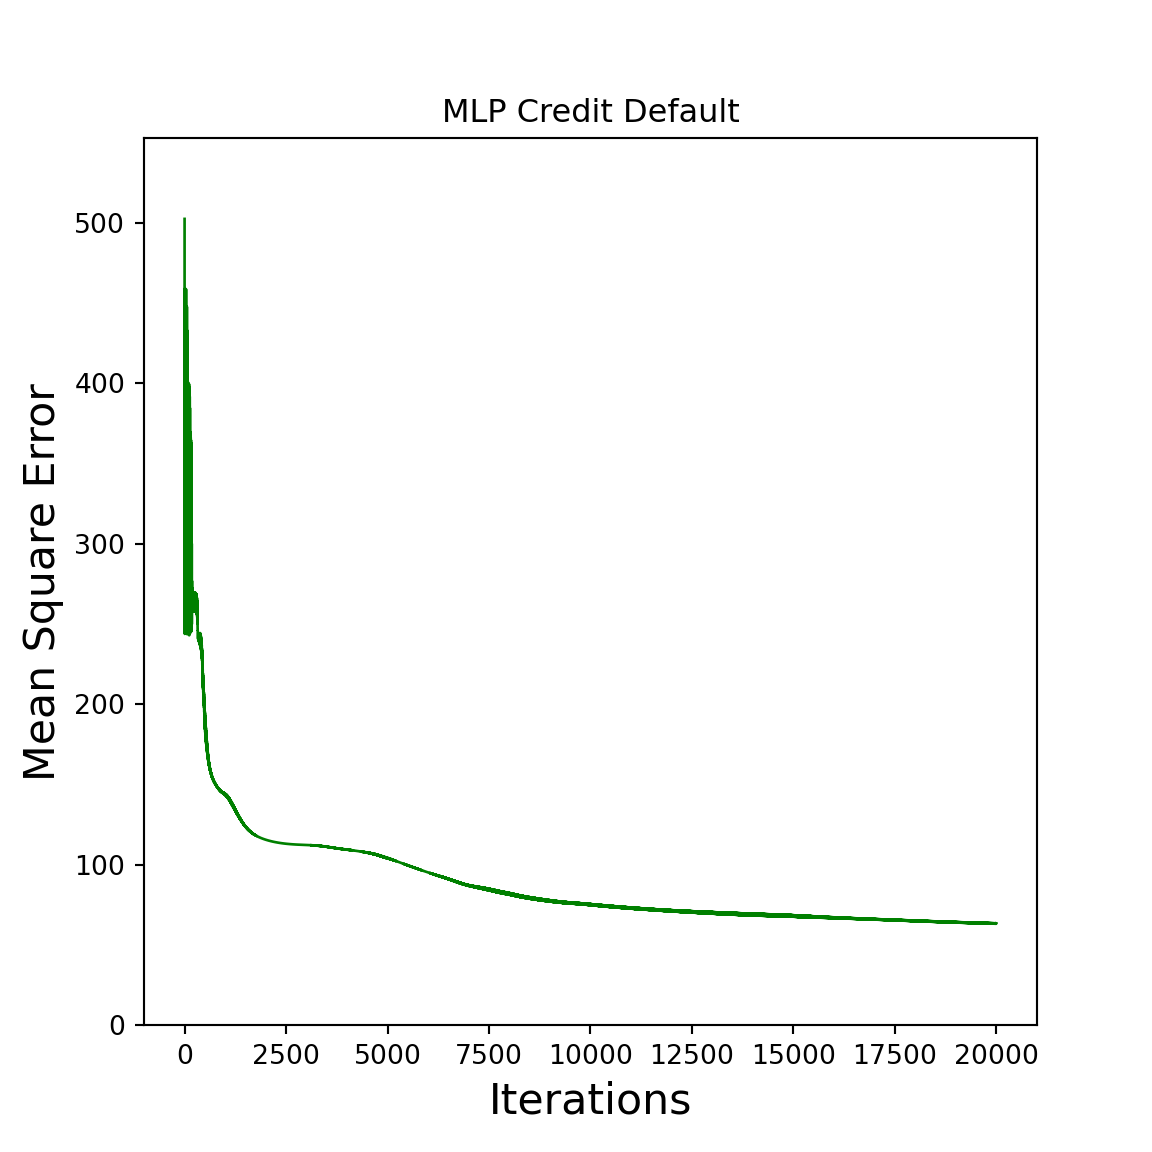
\includegraphics{gitbook-demo_files/figure-latex/unnamed-chunk-3-7.pdf}

\begin{verbatim}
## Mean Square error over all testdata:  2135.358966722297
## Mean Square error over all classified testdata:  2458.5
## Probability of a wrong output:  16.08 %
## Probability of a right output:  83.92 %
## array([[21463,  2843],
##        [ 2074,  4201]], dtype=int64)
\end{verbatim}

  \bibliography{book.bib,packages.bib}

\end{document}
